\documentclass[xcolor=x11names]{beamer}

\usetheme{EIS}

\usepackage{graphicx}
\usepackage{hyperref}
\usepackage{xspace}
\usepackage{attrib}
\usepackage{booktabs}
\usepackage{color}
\usepackage{ragged2e}
\usepackage{multicol}
\usepackage{multirow}
\usepackage[english]{babel}

\usepackage[backend=biber,style=authoryear-comp,natbib=true,isbn=false,url=false,doi=false,eprint=false,dashed=false]{biblatex}
\addbibresource{pmawhorter.bib}

\DeclareCiteCommand{\pcite}{}{\printfield{title} (\printnames{labelname} \printfield{year})}{,}{}

\usepackage{tikz}
\usetikzlibrary{arrows,shapes,backgrounds}

\usepackage{fontspec}
\defaultfontfeatures{Ligatures=TeX}
\newfontfeature{Microtype}{protrusion=default;expansion=default;}
%\setmainfont[Microtype]{Computer Modern Sans}
\usepackage{microtype}
%\setmainfont{Linux Libertine}
%\setsansfont{Linux Biolinum}

\usepackage{array}
\newcolumntype{L}[1]{>{\raggedright\let\newline\\\arraybackslash\hspace{0pt}}m{#1}}
\newcolumntype{C}[1]{>{\centering\let\newline\\\arraybackslash\hspace{0pt}}m{#1}}

\setbeamertemplate{navigation symbols}{}

\newcommand{\work}[1]{\textit{#1}\xspace}
\renewcommand*{\thefootnote}{\ensuremath{\ast}}
\newcommand{\cg}[1]{{\leavevmode\color{gray} #1}}
\newcommand{\pr}[1]{\texttt{#1}}
\newcommand{\prq}[2]{``\texttt{#1}{#2}''}

\newcommand{\ind}{\hspace*{0.8em}}
\newcommand{\svind}{\vspace*{0.3em}}
\newcommand{\vind}{\vspace*{0.5em}}

\def\dunyazad/{\textit{Dunyazad}}
\def\minstrel/{\textit{Minstrel}}
\def\skald/{\textit{Skald}}
\def\problemplanets/{\textit{Problem Planets}}
\def\facade/{\textit{Fa\c{c}ade}}


\title[AI for Understanding Narrative Choices] 
{%
Artificial Intelligence as a Tool for Understanding Narrative Choices%
}

\author[Mawhorter]
{%
  Peter~Mawhorter
}

\institute[UCSC]
{%
  Department of Computer Science \\
  University of California Santa Cruz
}

\date[2016-3-3]
{%
  March 3rd, 2016
}

\begin{document}

\begin{frame}
  \titlepage
\end{frame}

\begin{frame}{Narrative Choices}
\begin{center}
  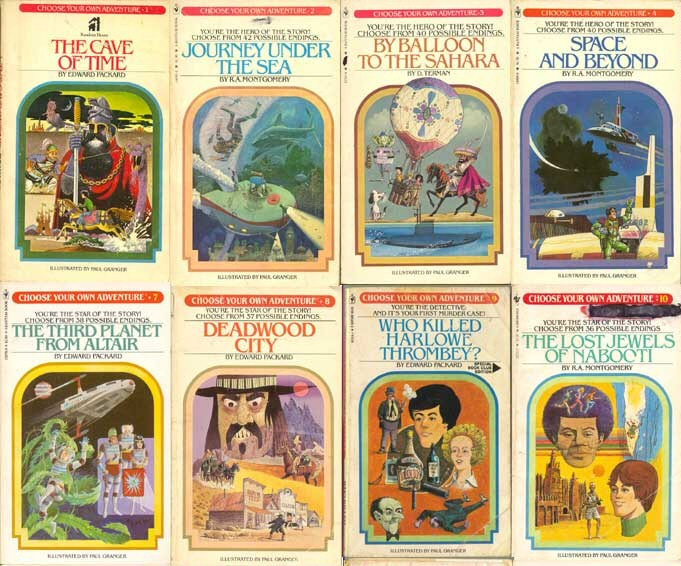
\includegraphics[width=0.8\textwidth]{res/cyoa-covers.jpg}
\end{center}
\end{frame}

\begin{frame}{Narrative Choices}
\begin{center}
  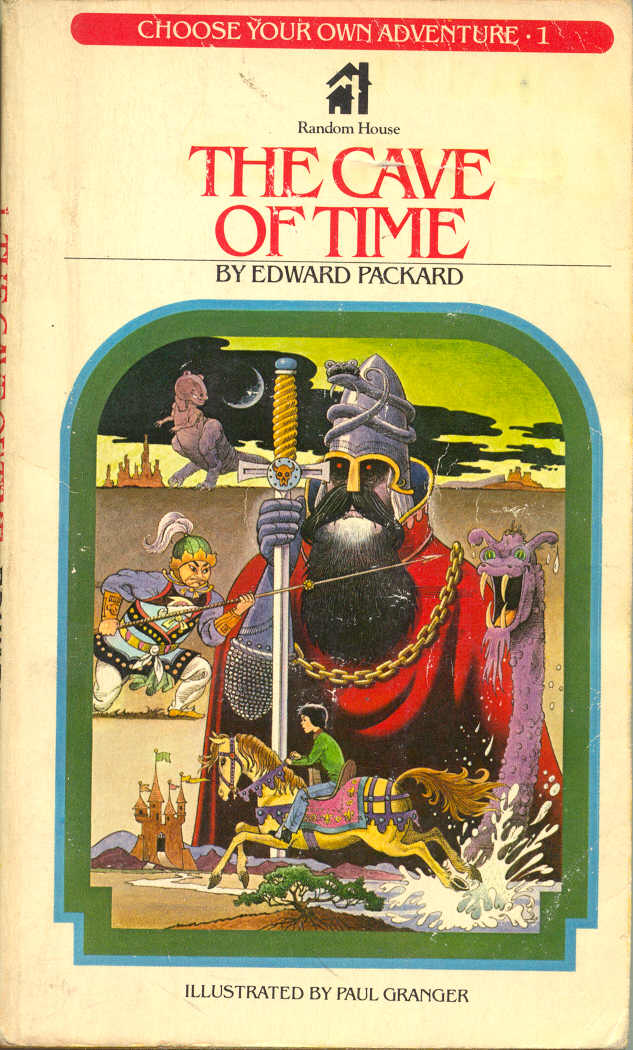
\includegraphics[height=0.8\textheight]{res/cave-of-time-cover.jpg}
  \hspace*{2em}
  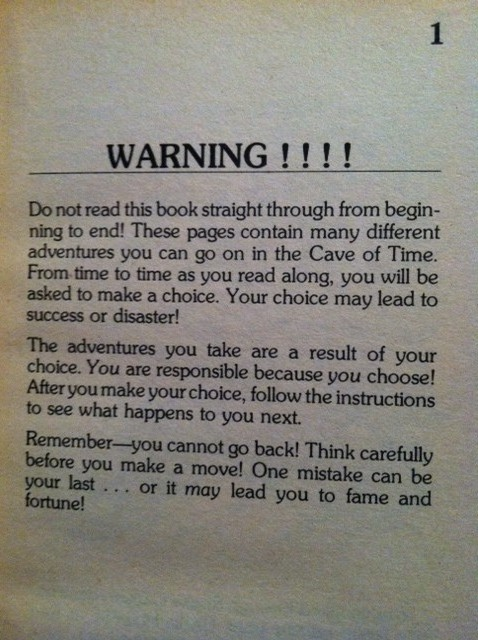
\includegraphics[height=0.8\textheight]{res/cave-of-time-warning.jpg}
\end{center}
\end{frame}

\begin{frame}{Motivation}
\begin{center}
  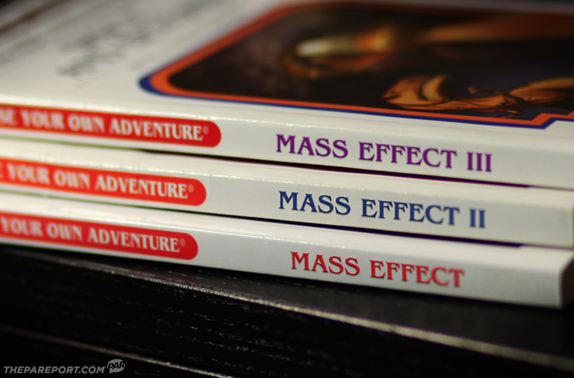
\includegraphics[width=0.95\textwidth]{res/mass-effect-cyoa.jpg}
\end{center}
\end{frame}

\begin{frame}{Motivation: Understanding Popular Culture}
\begin{center}
  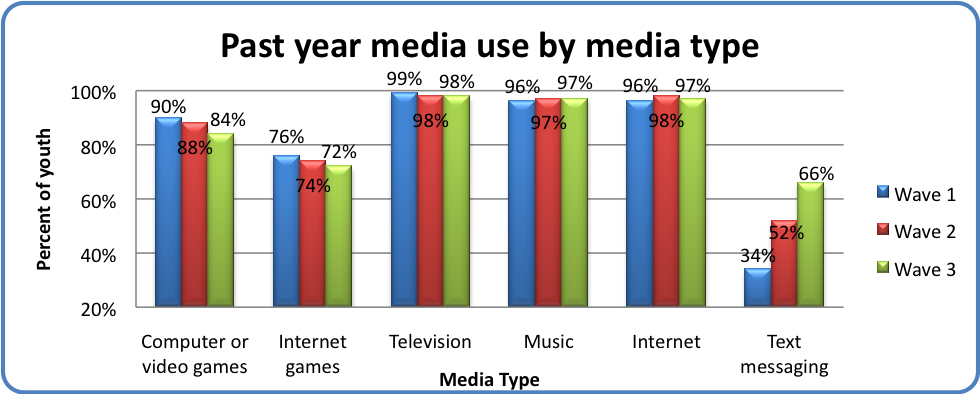
\includegraphics[width=\textwidth]{res/media-use-by-type.png} \\
  \vspace{1em}
  \tiny%
  Graph from the Growing Up With Media longitudinal study 2006--2008; participants were 10--15 years old. \\
  \vspace{1em}
  Published by the Center for Innovative Public Health Research \\
  \vspace{1em}
  \url{https://innovativepublichealth.org/bulletins/growing-up-with-media-media-use-patterns/}
\end{center}
\end{frame}

\begin{frame}{Motivation: Understanding Literature...}
\begin{center}
  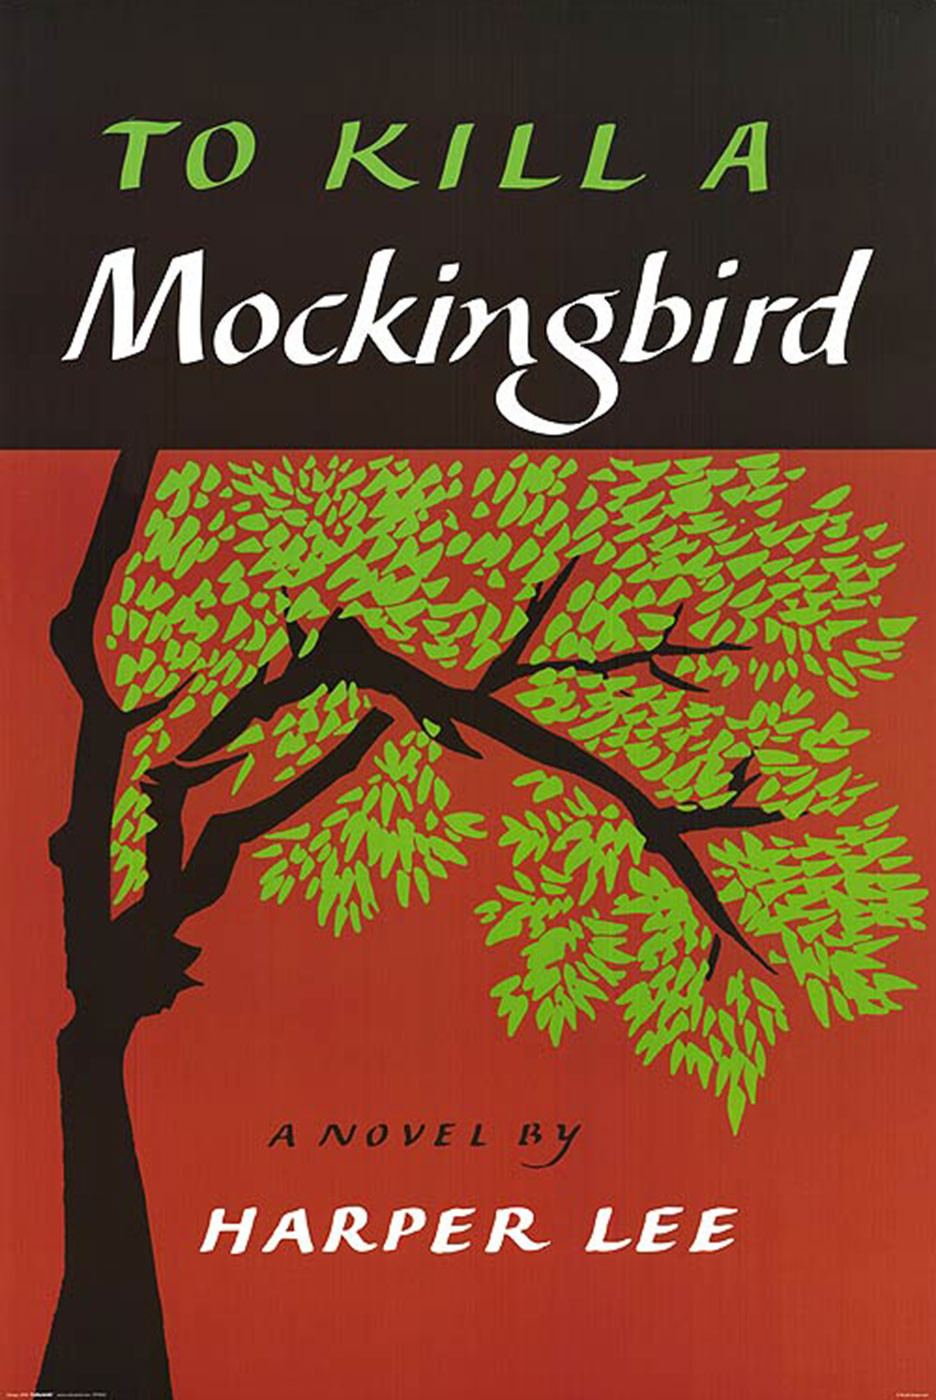
\includegraphics[height=0.8\textheight]{res/to-kill-a-mockingbird-cover.jpg}
  \hspace*{2em}
  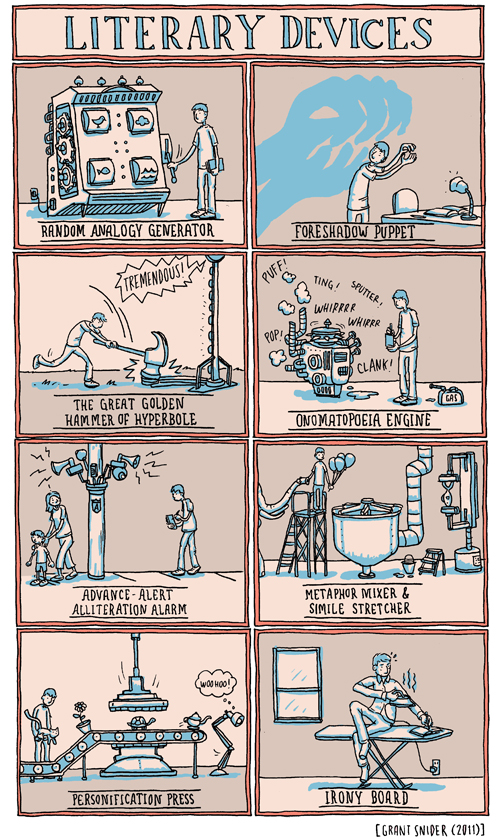
\includegraphics[height=0.8\textheight]{res/literary-devices.jpg}
\end{center}
\end{frame}

\begin{frame}{Motivation: Understanding Games?}
\begin{center}
  
\includegraphics[height=0.45\textheight]{res/journey-title.png}
  \hspace*{1em}
  
\includegraphics[height=0.45\textheight]{res/that-dragon-cancer.png}
  \vspace{1em}
  What can we say about how to understand and interpret these?
\end{center}
\end{frame}

\begin{frame}{Motivation: AI and Society}
\begin{center}
  
\includegraphics[height=0.4\textheight]{res/siri.png}
  \hspace*{1em}
  
\includegraphics[height=0.4\textheight]{res/facebook-ai-research.png}
  \hspace*{1em}
  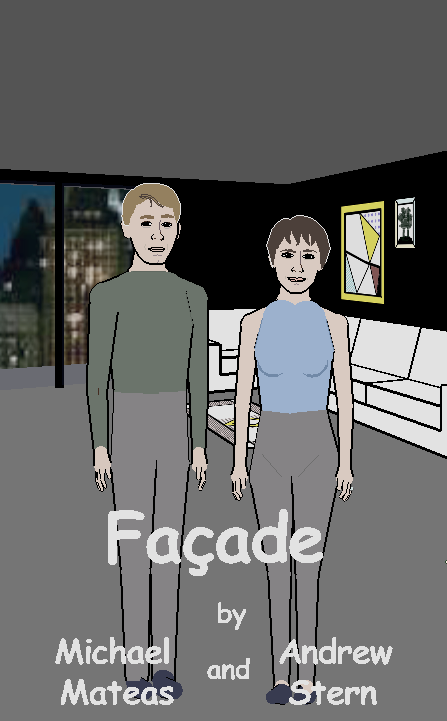
\includegraphics[height=0.4\textheight]{res/facade-title.png} \\
  \vspace{1em}
  If AI is enabling new media and modes of communication, can it also help us understand them?
\end{center}
\end{frame}

\begin{frame}{My Thesis}
  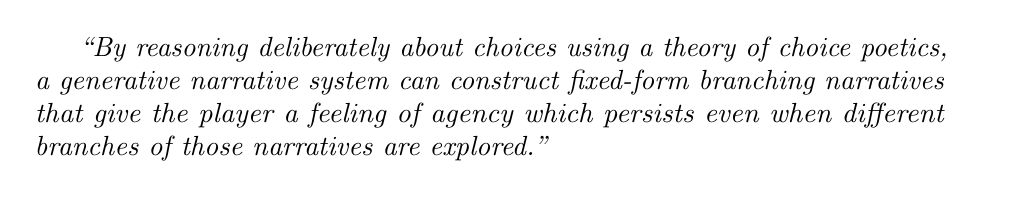
\begin{tikzpicture}
    \node(t)[text width=\textwidth] at (0,0) {%
      \parbox{0.95\textwidth}{
  \justifying%
  \itshape%
``By reasoning deliberately about choices using a theory of choice poetics, a generative narrative system can construct fixed-form branching narratives that give the player a feeling of agency which persists even when different branches of those narratives are explored.''%
    }};
  \end{tikzpicture}
\end{frame}

\begin{frame}{My Thesis}
  \vspace*{-0.05ex}%
  \hspace*{-0.25ex}%
  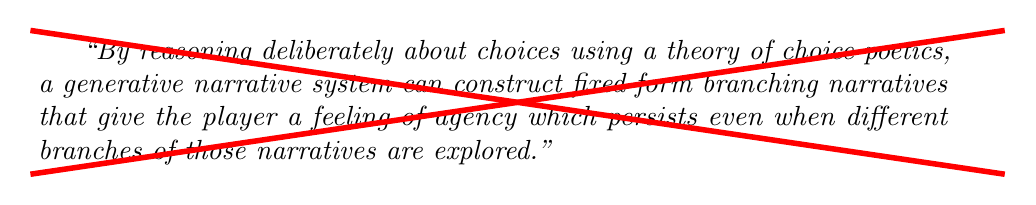
\begin{tikzpicture}
    \node(t)[text width=\textwidth] at (0,0) {%
      \parbox{0.95\textwidth}{
  \justifying%
  \itshape%
``By reasoning deliberately about choices using a theory of choice poetics, a generative narrative system can construct fixed-form branching narratives that give the player a feeling of agency which persists even when different branches of those narratives are explored.''%
    }};
    \draw[color=red,line width=2pt] (t.north west) -- (t.south east);
    \draw[color=red,line width=2pt] (t.south west) -- (t.north east);
  \end{tikzpicture}
\end{frame}

\begin{frame}{My Thesis}
  \justifying
  \itshape
  ``The simultaneous development of a theory for analyzing choice poetics and a system that operationalizes said theory to generate narrative choices provides benefits for both the system and the theory. This novel combination of critical and technical concerns has resulted in an original generative system as well as an analysis framework for understanding choices in terms of player goals.''
\end{frame}

\begin{frame}{My Thesis}
  \justifying
  \itshape
  ``The simultaneous development of a theory for analyzing choice poetics and a system that operationalizes said theory to generate narrative choices provides benefits for both the system and the theory.This \textbf{novel combination of critical and technical concerns} has resulted in an original generative system as well as an analysis framework for understanding choices in terms of player goals.''
\end{frame}

\begin{frame}{My Thesis}
  \justifying
  \itshape
  ``The simultaneous development of a theory for analyzing choice poetics and a system that operationalizes said theory to generate narrative choices provides benefits for both the system and the theory. This novel combination of critical and technical concerns has resulted in \textbf{an original generative system} as well as an analysis framework for understanding choices in terms of player goals.''
\end{frame}

\begin{frame}{My Thesis}
  \justifying
  \itshape
  ``The simultaneous development of a theory for analyzing choice poetics and a system that operationalizes said theory to generate narrative choices provides benefits for both the system and the theory. This novel combination of critical and technical concerns has resulted in an original generative system as well as \textbf{an analysis framework for understanding choices in terms of player goals}.''
\end{frame}

\begin{frame}{Outline}
  \begin{itemize}
    \item Motivation
    \item \textbf{Inspiration: \skald/ and \problemplanets/}
    \item \textbf{Methodology}
    \item \textbf{Related Work}
    \item \textbf{Theory: Choice Poetics}
    \item \textbf{Application: \dunyazad/}
    \item \textbf{Results: Options}
    \item \textbf{Results: Outcomes}
    \item \textbf{Conclusions}
  \end{itemize}
\end{frame}

\begin{frame}{\minstrel/}
  \justifying
  \setlength{\parindent}{1.5em}
  \itshape
  It was the spring of 1089, and a knight named Lancelot returned to Camelot from elsewhere. Lancelot was hot tempered. Once, Lancelot had lost a joust. Because he was hot tempered, Lancelot wanted to destroy his sword. Lancelot struck his sword. His sword was destroyed.

  One day, a lady of the court named Andrea wanted to have some berries\ldots
\end{frame}

\begin{frame}{\minstrel/}
  \vfill
  \begin{itemize}\addtolength{\itemsep}{0.5\baselineskip}
    \item Case-based story generation.
    \item Models human creativity through `Transform-Recall-Adapt Methods' (TRAMs).
    \item Manages story construction via `Author-Level Plans' (ALPs).
  \end{itemize}
  \vfill
  \centering
  \tiny
  \pcite{Turner1993}
\end{frame}

\begin{frame}{\skald/}
  \vfill
  \begin{itemize}\addtolength{\itemsep}{0.5\baselineskip}
    \item A rational reconstruction of \minstrel/.
    \item Focused on the TRAMs for imaginative recall.
    \item We experimented with different TRAM and ALP setups.
  \end{itemize}
  \vfill
  \centering
  \tiny
  \pcite{Tearse2014}
\end{frame}

\begin{frame}{\skald/: Experiments}
  \begin{itemize}\addtolength{\itemsep}{0.5\baselineskip}
    \item Results:
    \begin{itemize}\addtolength{\itemsep}{0.5\baselineskip}
      \vspace{0.5\baselineskip}
      \item TRAM configurations can trade coherence against variety.
      \item Modified boredom and TRAM selection can reduce search effort but also creativity.
    \end{itemize}
  \end{itemize}
  \vspace{1ex}
  \begin{tabular}{p{0.45\textwidth} p{0.45\textwidth}}
  \scriptsize
  \centering
  TRAM experiment: \newline
  \begin{tabular}{r c c}
      \toprule
      measure & orig. & mod. \\
      \midrule
      coherence & 35\% & 92\%  \\
      unique & 69 & 12 \\
      variation & 6.9 & 3.1  \\
      \bottomrule
  \end{tabular}
  &
  \scriptsize
  \centering
  Full system experiment: \newline
  \begin{tabular}{r c c}
      \toprule
      measure & orig. & mod. \\
      \midrule
      direct matches & 59\% & 72\% \\
      TRAMs tried & 13.8 & 7.7  \\
      TRAMs used & 2.4 & 1.4  \\
      \bottomrule
  \end{tabular} \newline
\end{tabular}
  \vfill
  \centering
  \tiny
  \pcite{Tearse2011} \\
  \pcite{Tearse2012}
\end{frame}

\begin{frame}{\problemplanets/}
  \begin{itemize}\addtolength{\itemsep}{0.5\baselineskip}
    \item A project to use \skald/ to build interactive vignettes.
    \item Vignettes would educate about climate change issues.
    \item The case library required delicate balancing.
    \item Coherence depended on complex ALPs.
    \item The placement of choices was static.
  \end{itemize}
\end{frame}

\begin{frame}{\problemplanets/}
  \begin{itemize}\addtolength{\itemsep}{0.5\baselineskip}
    \item Lessons:
    \begin{itemize}\addtolength{\itemsep}{0.5\baselineskip}
      \vspace{0.5\baselineskip}
      \item Focus on the consistency rules---raw material can be random.
      \item Come up with principles for placement and structure of choices.
    \end{itemize}
    \item $\rightarrow$ \dunyazad/
    \begin{itemize}\addtolength{\itemsep}{0.5\baselineskip}
      \vspace{0.5\baselineskip}
      \item A narrative generator focused on discrete choices.
      \item Uses answer-set programming to solve for story configurations.
    \end{itemize}
  \end{itemize}
\end{frame}

\begin{frame}{Outline}
  \begin{itemize}
    \item Motivation
    \item Inspiration: \skald/ and \problemplanets/
    \item \textbf{Methodology}
    \item \textbf{Related Work}
    \item \textbf{Theory: Choice Poetics}
    \item \textbf{Application: \dunyazad/}
    \item \textbf{Results: Options}
    \item \textbf{Results: Outcomes}
    \item \textbf{Conclusions}
  \end{itemize}
\end{frame}

\begin{frame}{Research Approach}
  \begin{itemize}\addtolength{\itemsep}{0.5\baselineskip}
    \item To intentionally construct choices requires goals and strategies:%
    \begin{itemize}\addtolength{\itemsep}{0.5\baselineskip}
      \vspace{0.5\baselineskip}
      \item Goals: poetic effects (e.g., obviousness).
      \item Strategies: a theory of choice poetics.
    \end{itemize}
    \item Existing theories are fragmented and focused elsewhere.
    \begin{itemize}\addtolength{\itemsep}{0.5\baselineskip}
      \vspace{0.5\baselineskip}
      \item Link poetics.
      \item Decision affect theory.
      \item Craft advice.
    \end{itemize}
  \end{itemize}
\end{frame}

\begin{frame}{Choice Poetics}
  \vfill
  \begin{itemize}\addtolength{\itemsep}{0.5\baselineskip}
      \item How do certain \textbf{choice structures} promote particular \textbf{poetic effects}?
    \begin{itemize}\addtolength{\itemsep}{0.5\baselineskip}
      \vspace{0.5\baselineskip}
      \item What is a \textbf{choice structure}?
      \item What \textbf{poetic effects} are possible?
      \item How do \textbf{player perspectives} affect the perception of choices?
    \end{itemize}
  \end{itemize}
  \vfill
  \centering
  \tiny
  \pcite{Mawhorter2014}
\end{frame}

\begin{frame}{Choice Poetics}
  \hspace*{-2em}%
  \begin{tabular}{p{1em} p{\textwidth}}
  \vspace{2.25em}
  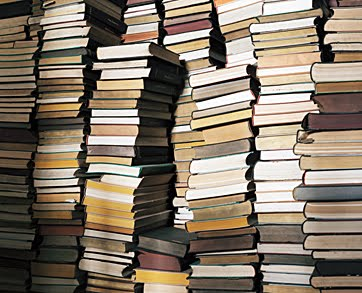
\includegraphics[width=3.5em]{res/stacked-books.jpg} \newline
  \vspace{2em}
  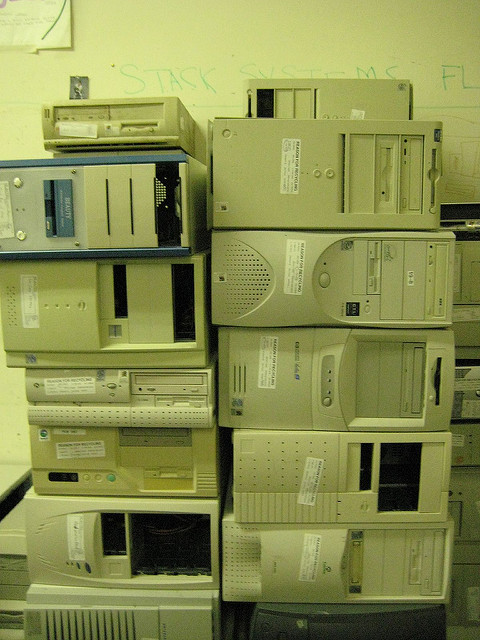
\includegraphics[width=3.5em]{res/stacked-computers.jpg}
  &
  \begin{itemize}\addtolength{\itemsep}{0.5\baselineskip}
      \item Classic approach: Carefully study existing narrative choices.
    \begin{itemize}\addtolength{\itemsep}{0.5\baselineskip}
      \vspace{0.5\baselineskip}
      \item Observe specific constructions and try to generalize them.
      \item Contrast works to show links between structure and poetics.
    \end{itemize}
    \item AI-based approach: Formalize intuitions and experiment.
    \begin{itemize}\addtolength{\itemsep}{0.5\baselineskip}
      \vspace{0.5\baselineskip}
      \item Express observed properties/relationships as logical rules.
      \item Generate choices which obey those rules.
      \item Add rules to correct/refine results.
      \item Translate added rules back into theoretical statements.
    \end{itemize}
    \pause
  \item \emph{Both approaches can inform each other.}
  \end{itemize}
  \end{tabular}
\end{frame}

\begin{frame}{Outline}
  \begin{itemize}
    \item Motivation
    \item Inspiration: \skald/ and \problemplanets/
    \item Methodology
    \item \textbf{Related Work}
    \item \textbf{Theory: Choice Poetics}
    \item \textbf{Application: \dunyazad/}
    \item \textbf{Results: Options}
    \item \textbf{Results: Outcomes}
    \item \textbf{Conclusions}
  \end{itemize}
\end{frame}

\begin{frame}{Related Work}
  \begin{itemize}\addtolength{\itemsep}{0.5\baselineskip}
    \item Criticism and Analysis
    \item Psychology and Cognitive Science
    \item Generative Systems
  \end{itemize}
\end{frame}

\begin{frame}{Criticism and Analysis}
  \begin{itemize}\addtolength{\itemsep}{0.5\baselineskip}
    \item Criticism and Analysis
    \begin{itemize}\addtolength{\itemsep}{0.5\baselineskip}
      \vspace{0.5\baselineskip}
      \item Formalist literary theory \\ \vspace{0.3\baselineskip}
        \tiny
        \pcite{Propp1971} \\
        \pcite{Barthes1975} \\
        \pcite{Greimas1988}

      \item \small Theories of Interactive Media \\ \vspace{0.3\baselineskip}
        \tiny
        \pcite{Murray1997} \\
        \pcite{Tosca1999} \\
        \pcite{WardripFruin2009} \\
        \pcite{Treanor2013} \\
        \pcite{Mitchell2012}

      \item \small Craft Advice \\ \vspace{0.3\baselineskip}
        \tiny
        \pcite{Laws2001} \\
        \pcite{ChoiceOfGamesChoiceRules}
    \end{itemize}
  \end{itemize}
\end{frame}

\begin{frame}{Psychology and Cognitive Science}
  \begin{itemize}\addtolength{\itemsep}{0.5\baselineskip}
    \item Psychology and Cognitive Science
    \begin{itemize}\addtolength{\itemsep}{0.5\baselineskip}
      \vspace{0.5\baselineskip}
      \item Specific effects (e.g., suspense; identification)\\ \vspace{0.3\baselineskip}
        \tiny
        \pcite{Gerrig1994} \\
        \pcite{Oatley1995}

      \item \small Science-informed criticism  \\ \vspace{0.3\baselineskip}
        \tiny
        \pcite{Palmer2004} \\
        \pcite{Zunshine2006}

      \item \small The psychology of decision-making \\ \vspace{0.3\baselineskip}
        \tiny
        \pcite{Tversky1993} \\
        \pcite{Mellers1999} \\
        \pcite{Schwartz2002}
    \end{itemize}
  \end{itemize}
\end{frame}

%\begin{frame}{Decision Affect Theory}
%\end{frame}

\begin{frame}{Generative Systems}
  \begin{itemize}\addtolength{\itemsep}{0.5\baselineskip}
    \item Generative Systems
    \begin{itemize}\addtolength{\itemsep}{0.5\baselineskip}
      \vspace{0.5\baselineskip}
      \item Effect-focused systems \\ \vspace{0.3\baselineskip}
        \tiny
        \pcite{Cheong2006} \\
        \pcite{Bae2008} \\
        \pcite{Ware2014}

      \item \small Interactive narrative systems \\ \vspace{0.3\baselineskip}
        \tiny
        \pcite{Szilas2003} \\
        \pcite{Barber2007a} \\
        \pcite{Yu2013}

      \item \small Player modelling \\ \vspace{0.3\baselineskip}
        \tiny
        \pcite{Mott2006} \\
        \pcite{Thue2008}
    \end{itemize}
  \end{itemize}
\end{frame}

%\begin{frame}{Dilemma-Based Interactive Fiction}
%\end{frame}

%\begin{frame}{Collaborative Filtering}
%\end{frame}

\begin{frame}{Outline}
  \begin{itemize}
    \item Motivation
    \item Inspiration: \skald/ and \problemplanets/
    \item Methodology
    \item Related Work
    \item \textbf{Theory: Choice Poetics}
    \item \textbf{Application: \dunyazad/}
    \item \textbf{Results: Options}
    \item \textbf{Results: Outcomes}
    \item \textbf{Conclusions}
  \end{itemize}
\end{frame}

\begin{frame}{Poetic Effects}
  \vfill
  \centering
  \begin{quote}
  \itshape
  The trees are in their autumn beauty, \\
  The woodland paths are dry, \\
  Under the October twilight the water \\
  Mirrors a still sky;
\end{quote}
\raggedleft
  -from \work{The Wild Swans At Coole} by William Butler Yeats \\
  \vfill
  \raggedright
  Broadly, \textbf{poetics} is the study of how literary techniques provoke audience reactions (the complement of hermeneutics).
\end{frame}

\begin{frame}{Poetic Effects}
  \centering
  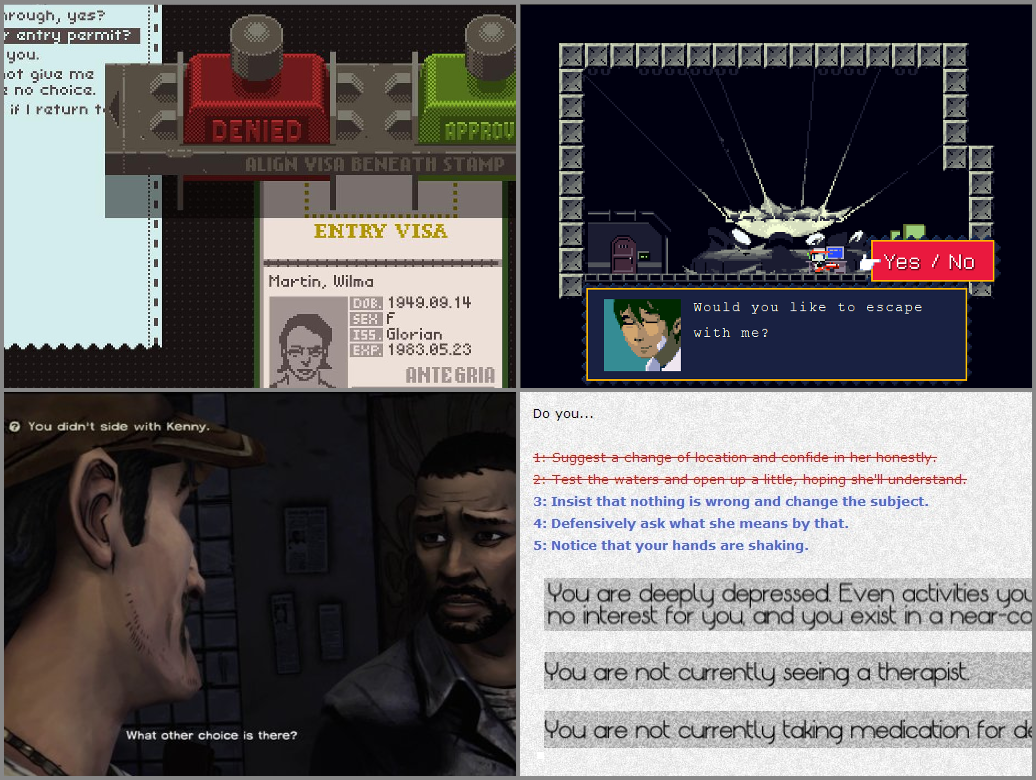
\includegraphics[height=0.8\textheight]{res/four-choices.png} \\
  \vspace{0.5ex}
  \textbf{Choice poetics} applies this to choices in narrative contexts.
\end{frame}

\begin{frame}{Choice Poetics}
  \vfill
  \begin{itemize}\addtolength{\itemsep}{0.5\baselineskip}
      \item How do certain \textbf{choice structures} promote particular \textbf{poetic effects}?
    \begin{itemize}\addtolength{\itemsep}{0.5\baselineskip}
      \vspace{0.5\baselineskip}
      \item What is a \textbf{choice structure}?
      \item What \textbf{poetic effects} are possible?
      \item How do \textbf{player perspectives} affect the perception of choices?
    \end{itemize}
  \end{itemize}
  \vfill
  \centering
  \tiny
  \pcite{Mawhorter2014}
\end{frame}

\begin{frame}{Choice Poetics}
  \begin{itemize}\addtolength{\itemsep}{0.5\baselineskip}
      \item \textbf{What is a choice?}
      \item \textbf{Modes of engagement}
      \item \textbf{Poetic effects}
      \item \textbf{Goal-based choice analysis}
  \end{itemize}
\end{frame}

\begin{frame}{Choice Structure}
  \begin{itemize}\addtolength{\itemsep}{0.5\baselineskip}
    \item Explicit, discrete choices:
    \begin{itemize}\addtolength{\itemsep}{0.5\baselineskip}
      \vspace{0.5\baselineskip}
      \item Framing
      \item Options
      \item Outcomes
      \begin{itemize}\addtolength{\itemsep}{0.5\baselineskip}
        \vspace{0.5\baselineskip}
        \item Outcome components
      \end{itemize}
    \end{itemize}
  \end{itemize}
\end{frame}

\begin{frame}{Choice Structure}
  \vspace{1ex}
  \begin{tabular}{p{0.15\textwidth} l}
    \vspace*{-0.5ex}
    \vtop{
      \null
      \hbox{\hspace{2em} framing $\left\{\rule{0pt}{14.5ex}\right.$}
      \hbox{\rule{0pt}{0.5ex}}
      \hbox{\hspace{2.2em} options $\left\{\rule{0pt}{3.5ex}\right.$\hspace*{-2ex}}
    }
    &
  \vtop{\null\hbox{%
  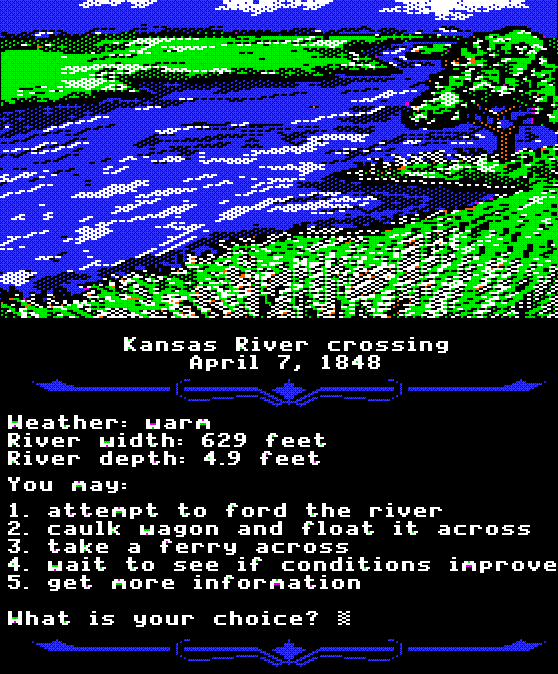
\includegraphics[width=0.5\textwidth]{res/oregon-trail-kansas-river-choice.png}
  }}
  \end{tabular}
\end{frame}

\begin{frame}{Choice Structure}
  \centering
  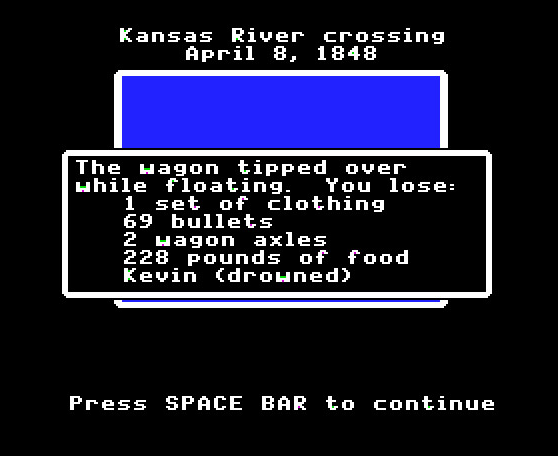
\includegraphics[width=0.5\textwidth]{res/oregon-trail-kansas-river-outcome.png} \\ \vspace{1ex}
  One possible outcome (with five apparent components).
\end{frame}

\begin{frame}{Choice Poetics}
  \begin{itemize}\addtolength{\itemsep}{0.5\baselineskip}
      \item What is a choice?
      \item \textbf{Modes of engagement}
      \item \textbf{Poetic effects}
      \item \textbf{Goal-based choice analysis}
  \end{itemize}
\end{frame}

\begin{frame}{Modes of Engagement}
  \hbox{
    \vtop{
      \null%
      \hbox{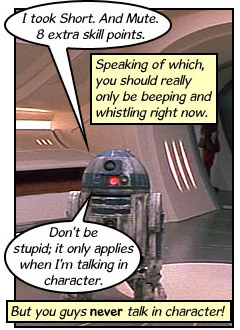
\includegraphics[width=0.28\textwidth]{res/r2d2minmax.jpg}}
    }
    \vtop{
      \null%
      \parbox{0.6\textwidth}{
      \begin{itemize}\addtolength{\itemsep}{0.5\baselineskip}
          \item \textbf{Reasons to play} are distinct from \textbf{reasons to decide}.
          \item Player goals determine how players evaluate options.
          \item \textbf{Modes of engagement} are frameworks for player goals.
      \end{itemize}
      }
    }
  }
\vfill
\tiny
\centering
\pcite{Yee2006} \\
\pcite{Kallio2011} \\
\pcite{Hamari2014}
\end{frame}

\begin{frame}{Modes of Engagement}
\vfill
\centering
\renewcommand*{\arraystretch}{1.5}
\scriptsize
\begin{tabular}{p{6em}p{12em}p{13em}}
\toprule
\textbf{Mode} & \textbf{Decision Process} & \textbf{Example} \\
\midrule
\textbf{Avatar Play} & Decide as if you were in the character's situation. & When picking a pet, pick the cat because you like cats. \\
\textbf{Role Play} & Decide in order to act out a persona. & Choose the wizard character class because you want to play a shy, bookish person. \\
\textbf{Power Play} & Choose options that advance game metrics like score, beating other players, or quick completion. & Sacrifice an ally to obtain a powerful item because it helps you beat the game more quickly. \\
\textbf{Exploratory Play} & Choose options to see what will happen. & Turn away from the path of your quest to explore the world. \\
\textbf{Social Play} & In a multiplayer situation, choose options because of social considerations. & Turn down a high-level quest in order to accompany your friend on a lower-level quest. \\
\bottomrule
\end{tabular} \\ \vspace{1ex}
\ldots and more, for example \textbf{analytical play} and \textbf{critical play}.
\end{frame}

\begin{frame}{Choice Poetics}
  \begin{itemize}\addtolength{\itemsep}{0.5\baselineskip}
      \item What is a choice?
      \item Modes of engagement
      \item \textbf{Poetic effects}
      \item \textbf{Goal-based choice analysis}
  \end{itemize}
\end{frame}

\begin{frame}{Poetic Effects}
  \centering
  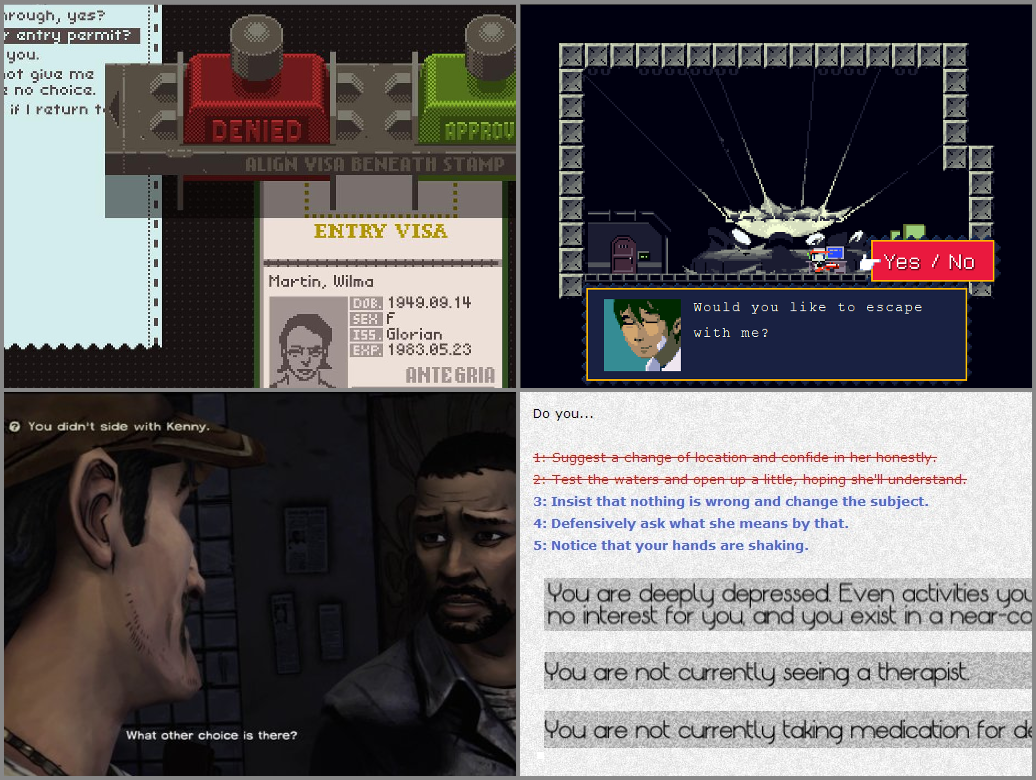
\includegraphics[height=0.8\textheight]{res/four-choices.png} \\
  \vspace{0.5ex}
  What audience reactions do these choices provoke?
\end{frame}

\begin{frame}{Poetic Effects}
  \begin{itemize}\addtolength{\itemsep}{0.5\baselineskip}
      \item \textbf{Identification} \\ \vspace{0.3\baselineskip}
      \small Viewing a character as a role model and/or as yourself.\\ \vspace{0.3\baselineskip}
      \tiny \pcite{Klimmt2009}

    \item \normalsize \textbf{Agency} \\ \vspace{0.3\baselineskip}
      \small A feeling of being in control and taking directed action. \\ \vspace{0.3\baselineskip}
      \tiny \pcite{WardripFruin2009} \\
      \tiny \pcite{Mason2013}

    \item \normalsize \textbf{Regret} \\ \vspace{0.3\baselineskip}
      \small Regret for an in-game action (as opposed to sympathy with a character who feels regret or being provoked to reminisce about a personal regret). \\ \vspace{0.3\baselineskip}
      \tiny \pcite{Frome2006} \\
      \tiny \pcite{Zagal2009}
  \end{itemize}
\end{frame}

\begin{frame}{Poetic Effects}
  \begin{itemize}\addtolength{\itemsep}{0.5\baselineskip}
      \item Other effects include \textbf{immersion}, \textbf{transportation}, \textbf{agency}, \textbf{influence}, \textbf{autonomy}, \textbf{responsibility} and more\ldots
      \item Choices don't determine these alone, but they can play an important role.
      \item These \emph{high-level} effects depend on \emph{low-level} effects such as being a dilemma or being obvious.
  \end{itemize}
\end{frame}

\begin{frame}{Choice Poetics}
  \begin{itemize}\addtolength{\itemsep}{0.5\baselineskip}
      \item What is a choice?
      \item Modes of engagement
      \item Poetic effects
      \item \textbf{Goal-based choice analysis}
  \end{itemize}
\end{frame}

\begin{frame}{Goal-Based Choice Analysis}
  \begin{itemize}\addtolength{\itemsep}{0.5\baselineskip}
    \item A framework for understanding choices in terms of \textbf{player goals}.
    \item It has \textbf{generative viability}: it has been shown to be sufficient for generating some kinds of choices.
    \item \dunyazad/ uses an automatic version to create choices.
  \end{itemize}
\end{frame}

\begin{frame}{Goal-Based Choice Analysis}
  \centering
  \begin{tabular}{p{0.45\textwidth} p{0.55\textwidth}}
  \vtop{
    \null
    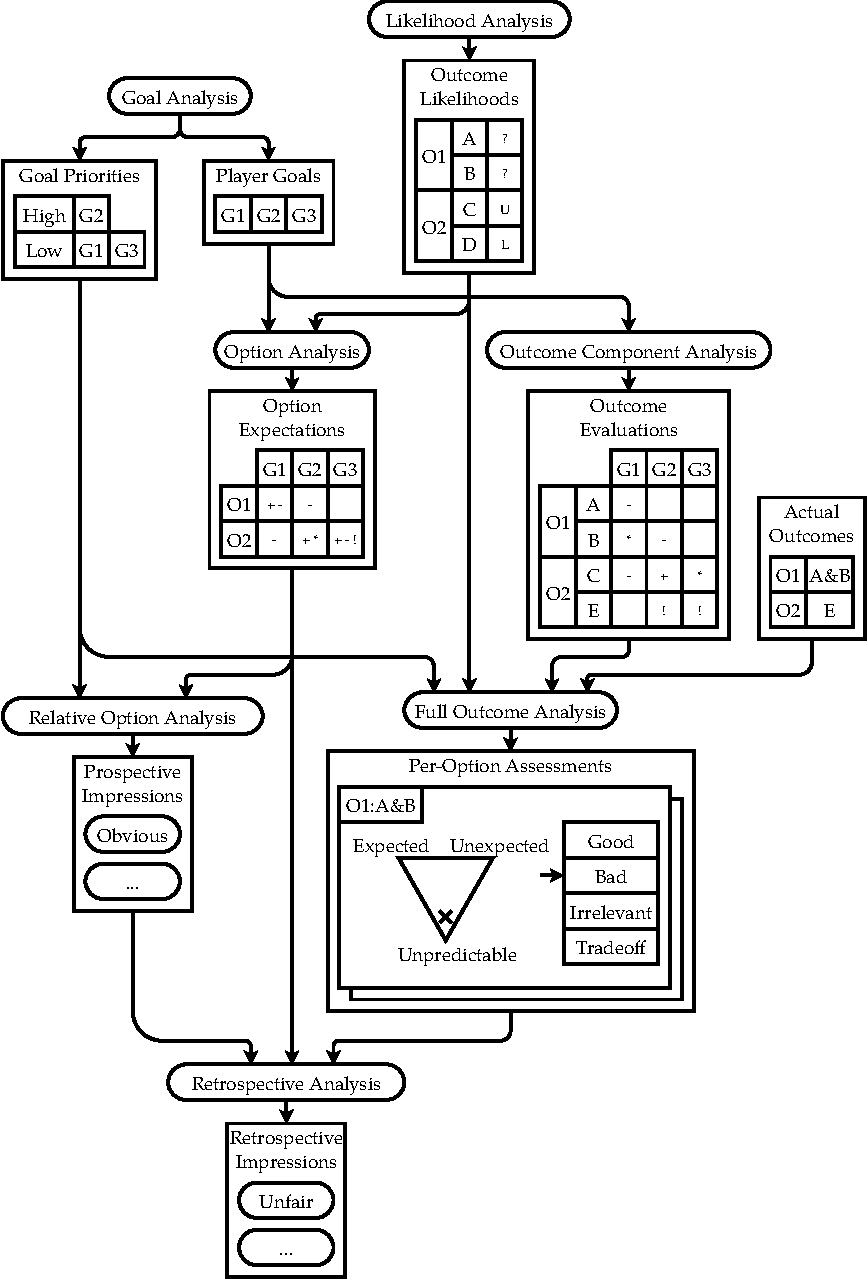
\includegraphics[width=0.45\textwidth]{fig/analysis-method-crop.pdf}
  }
  &
  \vspace{2em}
  \begin{enumerate}\addtolength{\itemsep}{0.5\baselineskip}
    \item Goal Analysis
    \item Likelihood Analysis
    \item Option Analysis
    \item Relative Option Analysis
    \item Outcome Component Analysis
    \item Full Outcome Analysis
    \item Retrospective Analysis
  \end{enumerate}
  \end{tabular}
\end{frame}

\begin{frame}{1. Goal Analysis}
  \begin{itemize}\addtolength{\itemsep}{0.5\baselineskip}
    \item Come up with an estimate of the player's goals. 
    \item Also estimate goal priorities.
    \item Without online player modelling, an authorial estimate of player goals must sufice.
    \item Multiple independent analyses can capture player groups with different modes of engagement.
  \end{itemize}
\end{frame}

\begin{frame}{An Example}
  \centering
  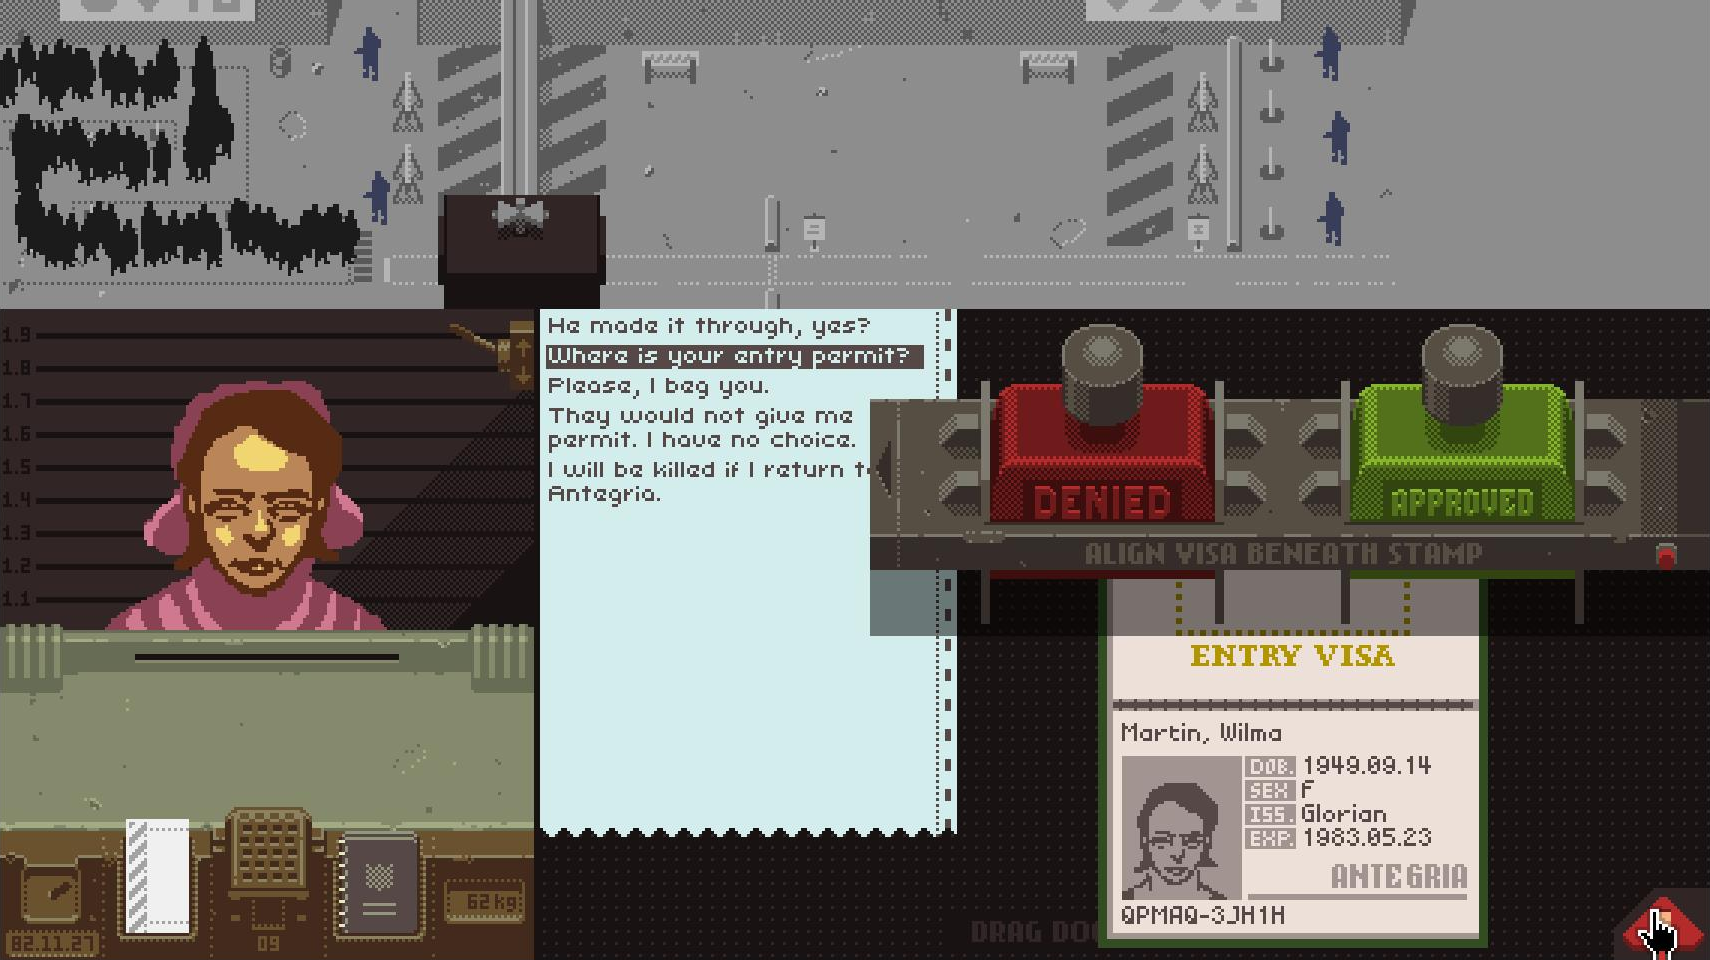
\includegraphics[width=\textwidth]{res/papersplease-large.png} \\
\end{frame}

\begin{frame}{Example: Goal Analysis}
  \centering
  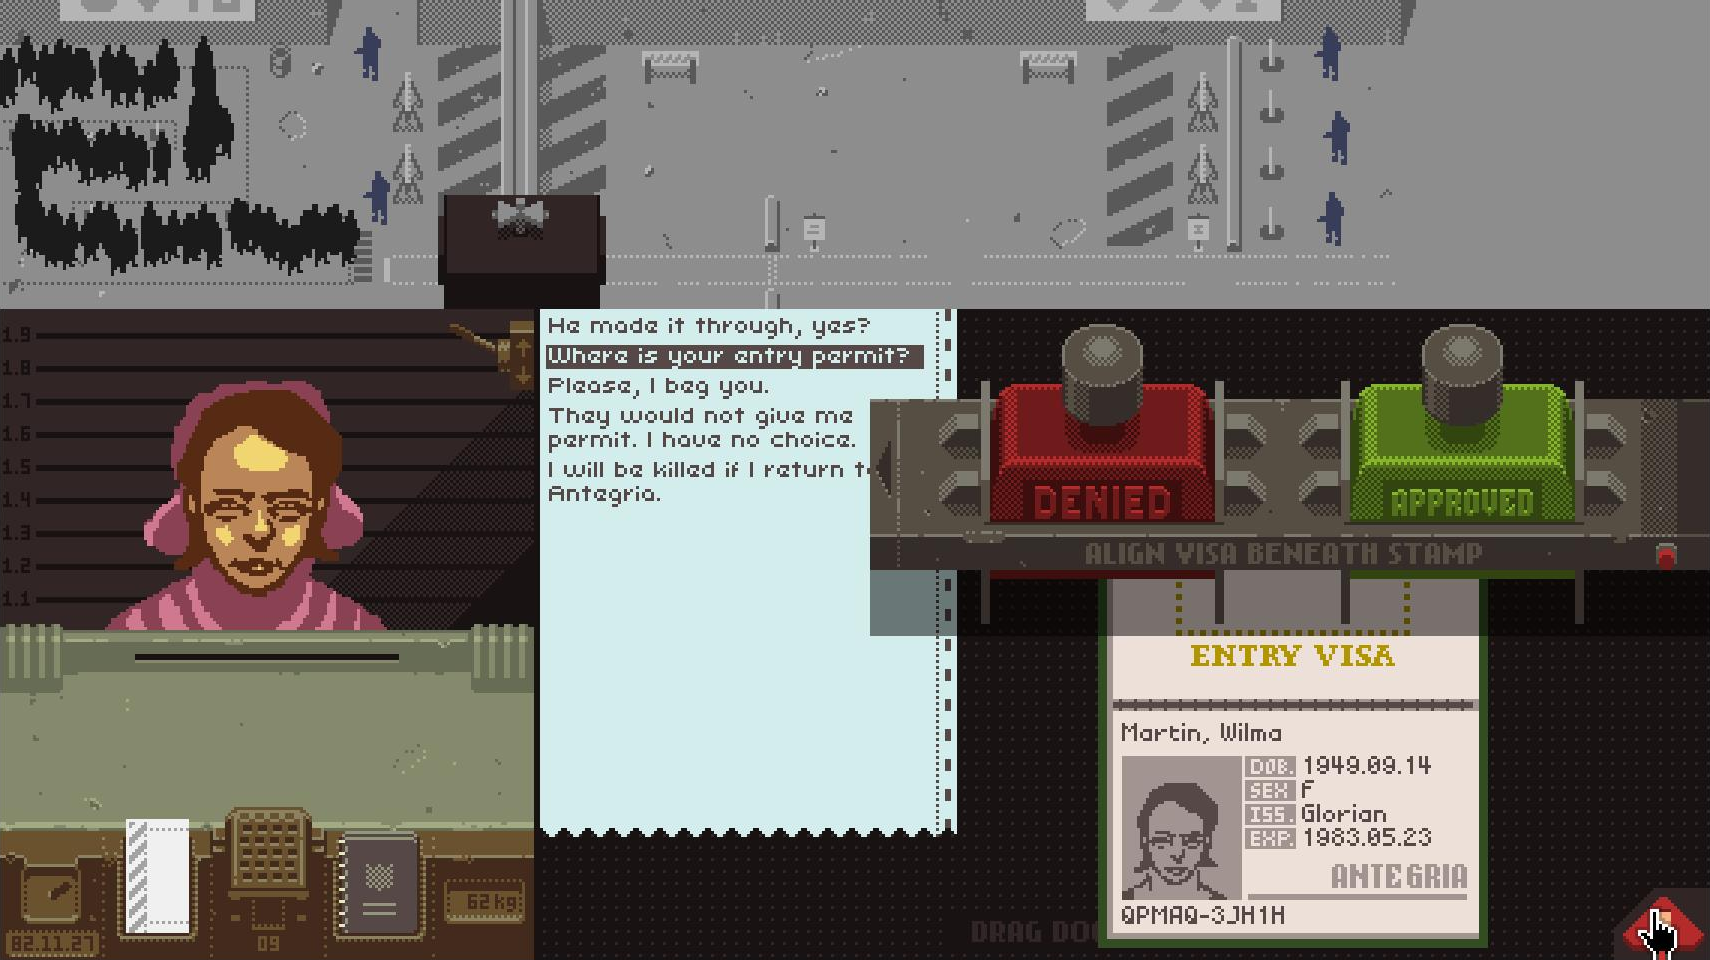
\includegraphics[height=0.3\textheight]{res/papersplease-large.png} \\
  \raggedright
  \begin{itemize}
    \item {[highest] Feed your family.}
    \item {[high] Avoid the penalty for making mistakes.}
    \item {[high] Treat travelers ethically.}
    \item {[medium] Prevent dishonest travelers from gaining entry.}
    \item {[low] Let approved travelers through.}
  \end{itemize}
\end{frame}

\begin{frame}{2. Likelihood Analysis}
  \begin{itemize}\addtolength{\itemsep}{0.5\baselineskip}
    \item Estimate the likelihood of each outcome component of every option.
    \item Only necessary when outcomes are nondeterministic.
    \item Estimate likelihoods \emph{from the player's perspective}.
    \item Again, multiple independent analyses can capture different player perspectives.
  \end{itemize}
\end{frame}

\begin{frame}{Example: Likelihood Analysis}
  \centering
  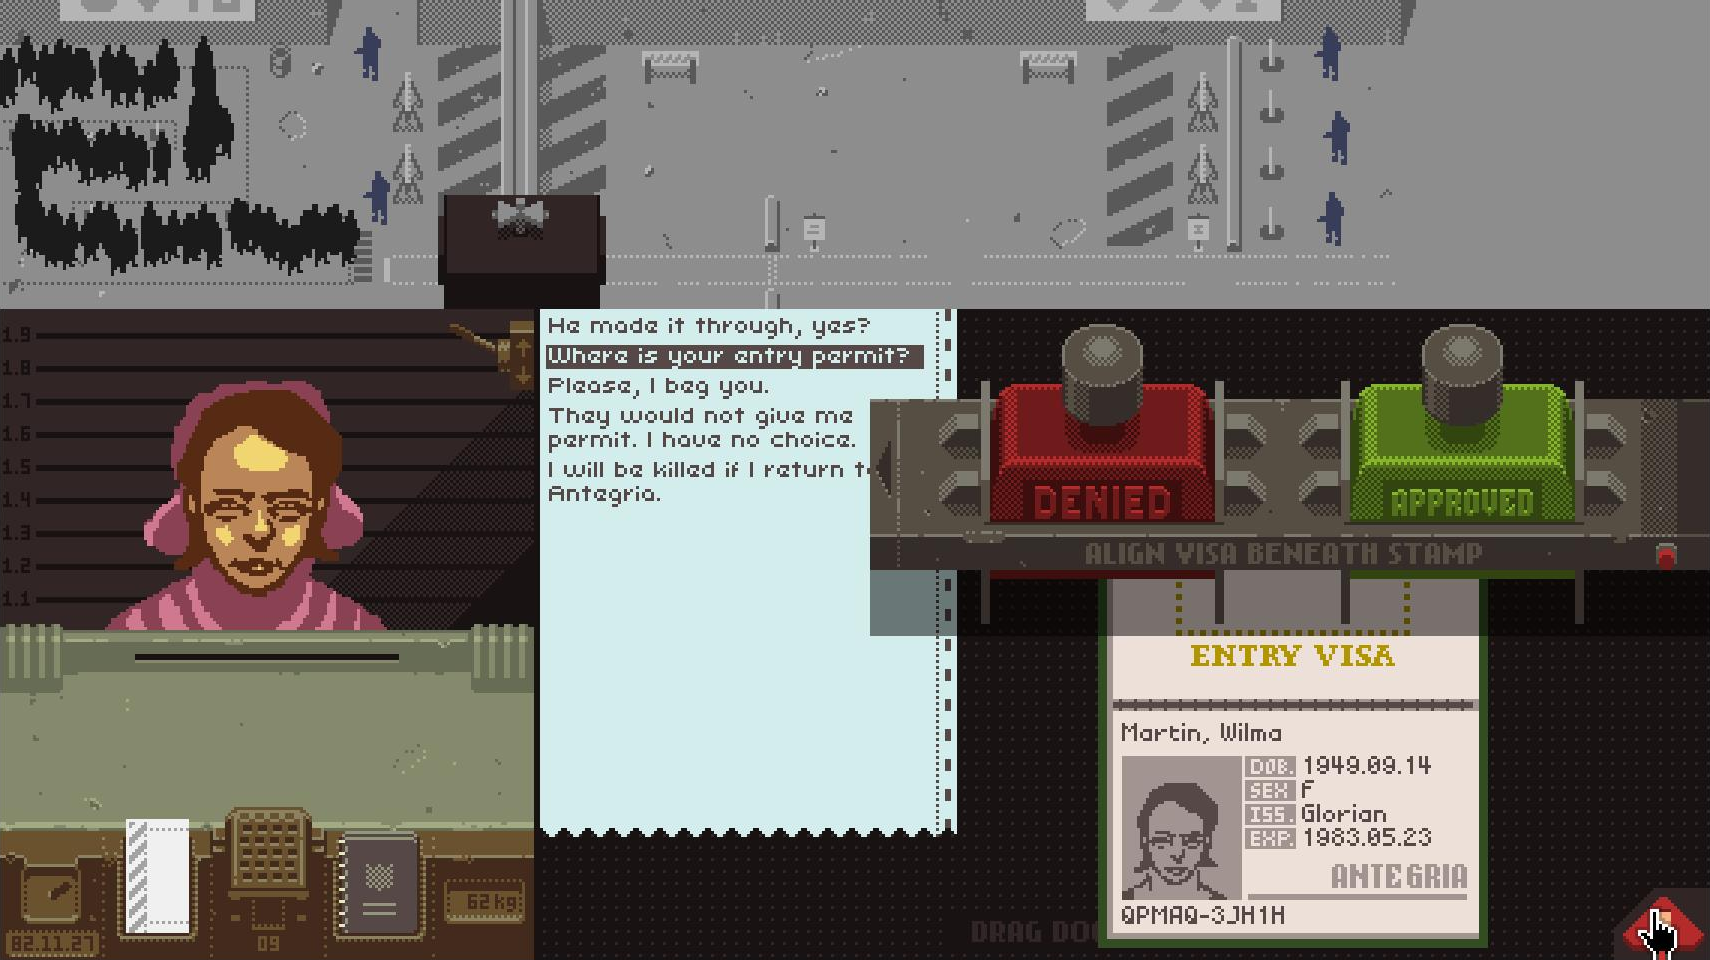
\includegraphics[height=0.3\textheight]{res/papersplease-large.png} \\
  \vspace*{1em}
  \small
  \begin{tabular}{l l}
    \toprule
    \multicolumn{1}{c}{\textbf{Approve}} & \multicolumn{1}{c}{\textbf{Deny}} \\
    \midrule
    {[likely] `Mistake' is discovered.} & [likely] No mistake is possible. \\
    {[unknown] Traveler is saved.} & [unknown] Traveler will be killed. \\
    {[unknown] Crminal gains entry.} & [unknown] Criminal is stymied. \\
    {[unlikely] Earn a credit.} & [likely] Earn a credit. \\
    \bottomrule
  \end{tabular}
\end{frame}

\begin{frame}{3. Option Analysis}
  \begin{itemize}\addtolength{\itemsep}{0.5\baselineskip}
    \item Given outcome likelihoods and player goals, estimate the perceived effect of each option on each goal.
    \item Per option/goal, look for positive or negative effects and whether they're likely or merely possible.
  \end{itemize}
  \vfill
  \centering
  \begin{tabular}{r c c}
    \toprule
           & Possible & Likely \\
    \midrule
    Positive    & \textbf{Enables}  & \textbf{Advances} \\
    Negative & \textbf{Threatens} & \textbf{Hinders} \\
    \bottomrule
  \end{tabular}
  \vfill
  \raggedright
  \begin{itemize}\addtolength{\itemsep}{0.5\baselineskip}
    \item Multiple overlapping assignments are possible (e.g., a choice that \textbf{enables}, \textbf{threatens}, \emph{and} \textbf{hinders} a particular goal).
  \end{itemize}
\end{frame}

\begin{frame}{Example: Option Analysis}
  \centering
  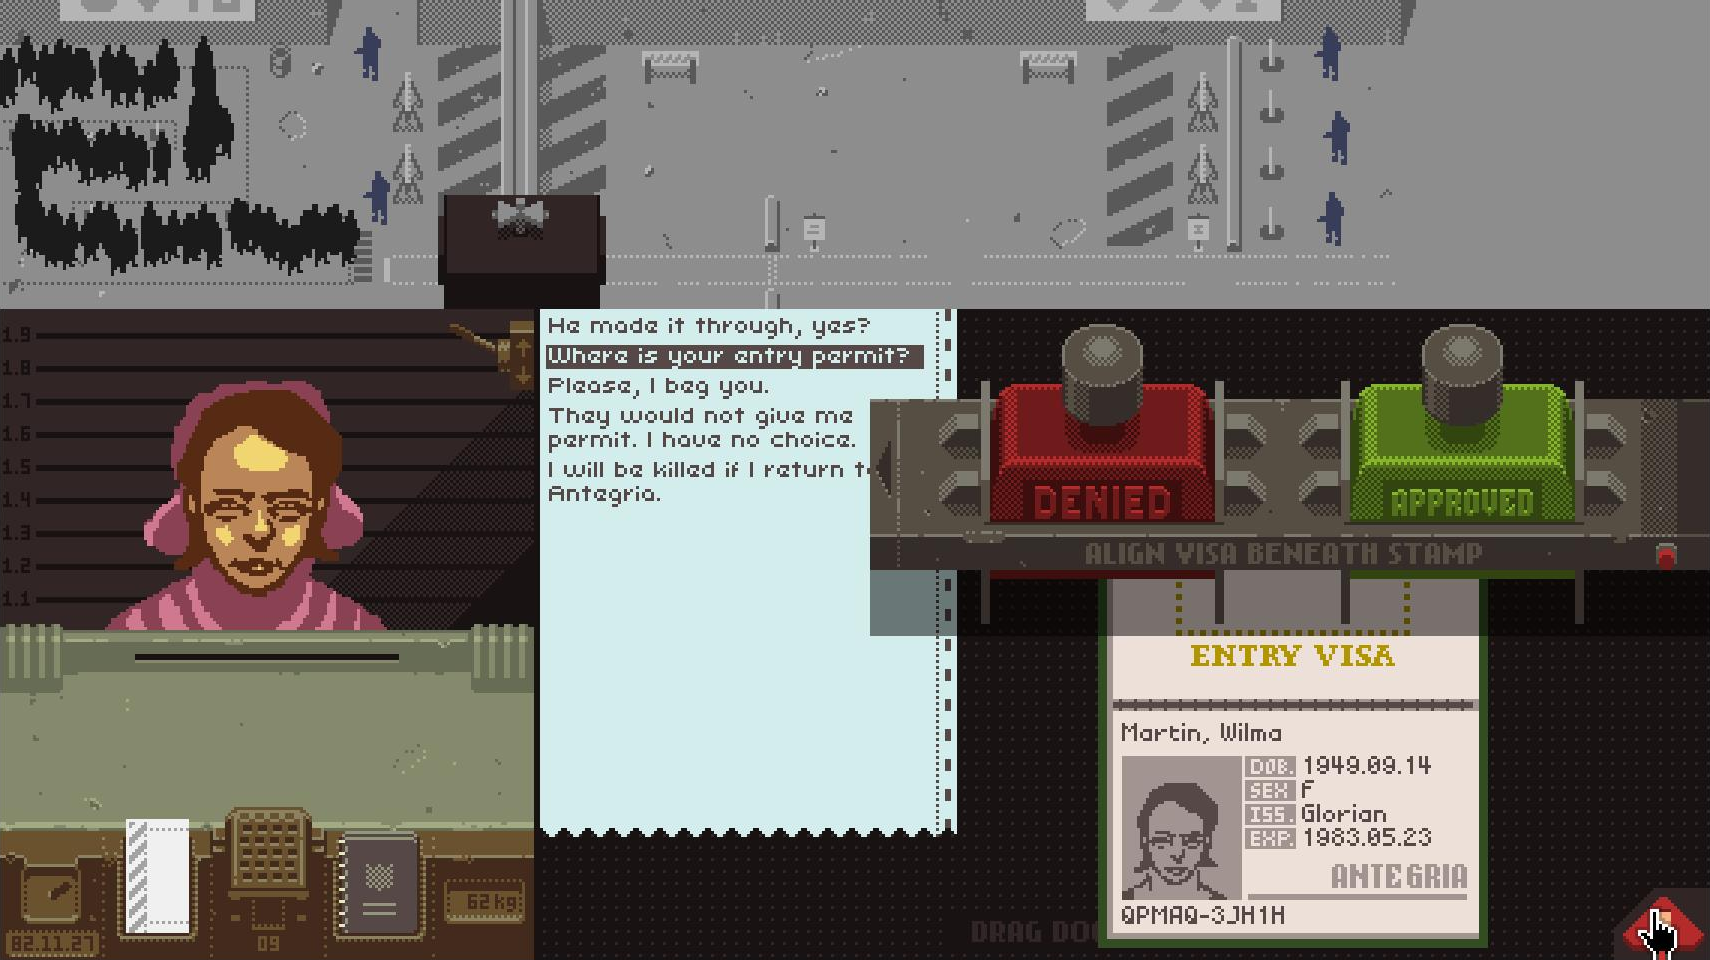
\includegraphics[height=0.3\textheight]{res/papersplease-large.png} \\
  \vspace*{0.2em}
  \footnotesize
  \begin{tabular}{c c c}
    \toprule
    \textbf{Goal} & \textbf{Approve} & \textbf{Deny} \\
    \midrule
    \multirow{3}{*}{<feed your family>} & \textbf{enables} & \textbf{enables} \\
                                        & \textbf{threatens} & \\
                                        & \textbf{hinders} & \textbf{advances} \\
    \midrule

    \multirow{3}{*}{<avoid penalty>} & \textbf{enables} & \textbf{enables} \\
                                     & \textbf{threatens} & \\
                                     & \textbf{hinders} & \textbf{advances} \\
    \midrule

    \multirow{2}{*}{<treat ethically>} & \textbf{enables} & \textbf{enables} \\
                                       & & \textbf{threatens} \\
    \midrule

    <stop cheaters> & \textbf{threatens} & \textbf{enables} \\
    \bottomrule
  \end{tabular}
\end{frame}

\begin{frame}{4. Relative Option Analysis}
  \begin{itemize}\addtolength{\itemsep}{0.5\baselineskip}
    \item Given goal priorities and the results of option analysis, categorize the set of options.
    \item Some structures such as a \textbf{dilemma} or an \textbf{obvious} choice may be immediately recognizeable.
    \item Other structures can be compared to well-understood cases.
  \end{itemize}
\end{frame}

\begin{frame}{4. Relative Option Analysis}
\centering
\renewcommand*{\arraystretch}{1.5}
\footnotesize
\hspace*{-1.5em}
\begin{tabular}{p{4.5em}p{10em}p{18.5em}}
\toprule
\textbf{Label} & \textbf{Description} & \textbf{Criteria} \\
\midrule
\textbf{Dilemma} & A difficult decision between two negative outcomes. & Exactly two options, each of which \textbf{hinders} one of two different high-priority player goals. The priorities of the goals and the severity of the consequences should be balanced and neither option should \textbf{enable} or \textbf{advance} any goals (even low-priority ones). \\
\textbf{Obvious} & A choice that has one option which is clearly better than the rest. & One option that \textbf{advances} a high-priority player goal without \textbf{hindering} any (although it may \textbf{threaten} some), while none of the rest of the options \textbf{enable} any high-priority goals, and each of them \textbf{threatens} some goal. \\
\textbf{Relaxed} & A choice that has no impact on any high-priority goals and where no goals are threatened. & There are no option expectations involving high-priority goals (positive or negative), and there are no \textbf{threatens} expectations (and thus no \textbf{hinders} expectations). \\
\bottomrule
\end{tabular}
\end{frame}

\begin{frame}{4. Relative Option Analysis}
  \vfill
  \begin{itemize}\addtolength{\itemsep}{0.5\baselineskip}
    \item Only \emph{expected} outcomes are considered, not \emph{actual} outcomes.
    \item Resulting \textbf{prospective impressions} estimate players' perceptions of a choice before making a decision
    \item Some effects such as elevated tension via a series of difficult choices depend mainly on \textbf{prospective impressisons}.
  \end{itemize}
  \vfill
  \centering
  \scriptsize (My first experiment tested the \textbf{relaxed}, \textbf{obvious}, and \textbf{dilemma} impressions.)
\end{frame}

\begin{frame}{Example: Relative Option Analysis}
  \centering
  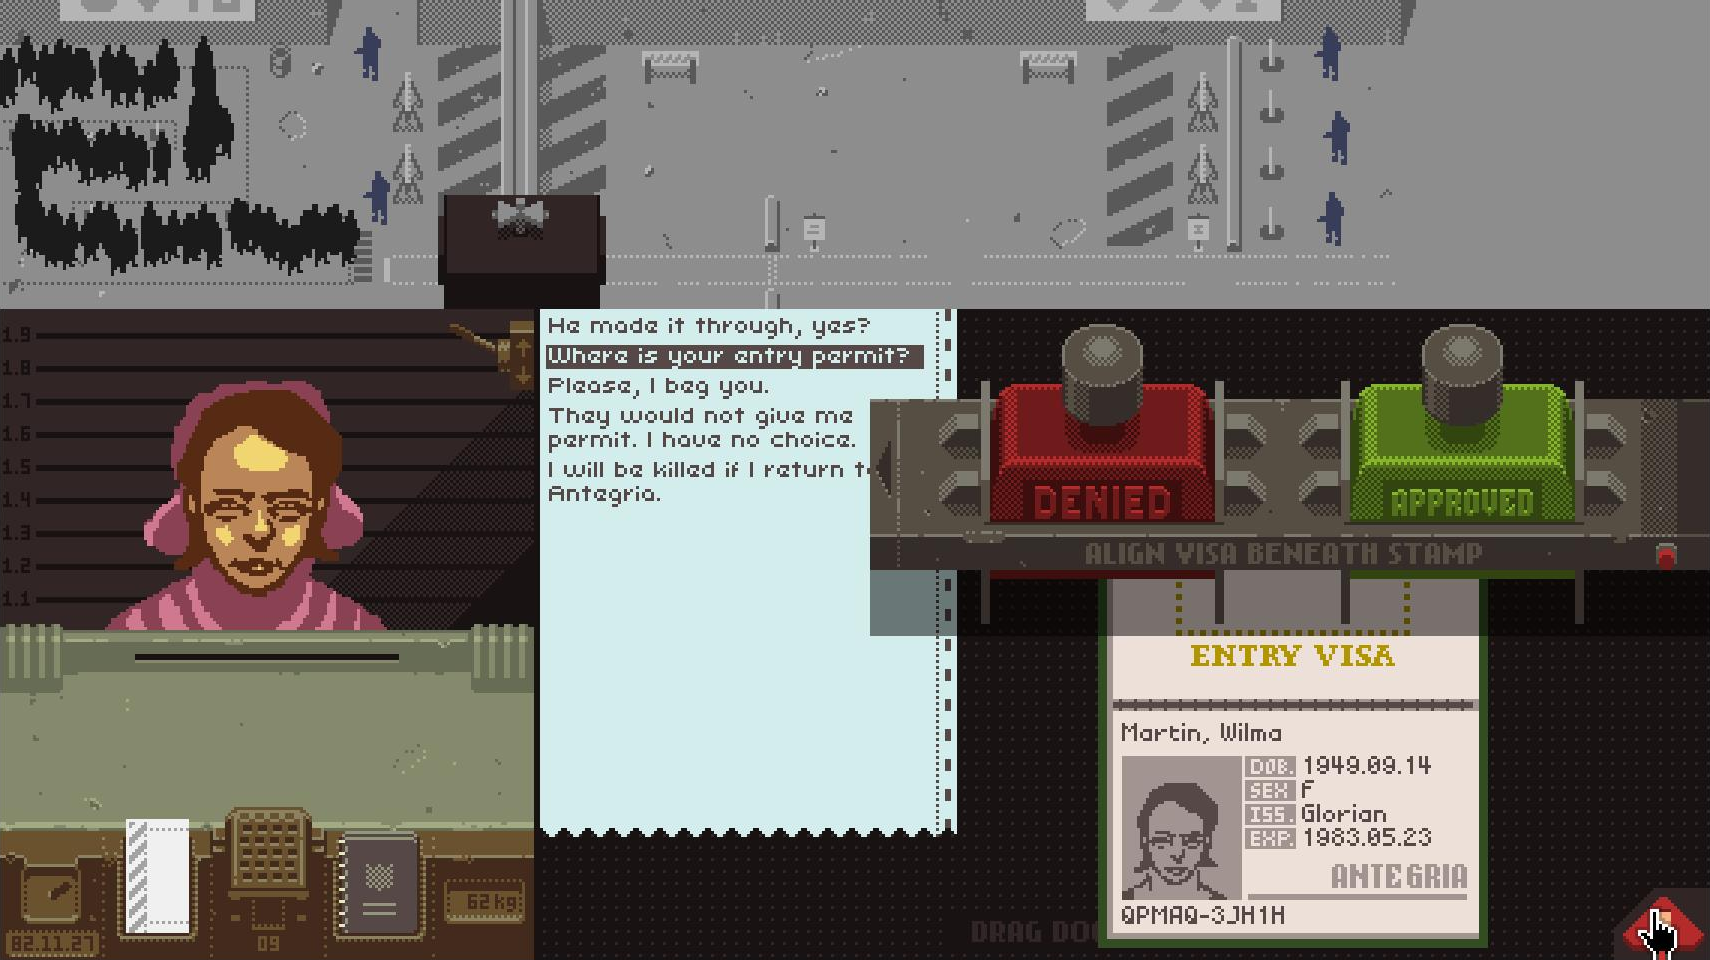
\includegraphics[height=0.3\textheight]{res/papersplease-large.png} \\
  \vspace*{0.2em}
  \footnotesize
  \begin{tabular}{c c c}
    \toprule
    \textbf{Goal} & \textbf{Approve} & \textbf{Deny} \\
    \midrule
    \multirow{3}{*}{<feed your family>} & \textbf{enables} & \textbf{enables} \\
                                        & \textbf{threatens} & \\
                                        & \textbf{hinders} & \textbf{advances} \\
    \midrule

    \multirow{3}{*}{<avoid penalty>} & \textbf{enables} & \textbf{enables} \\
                                     & \textbf{threatens} & \\
                                     & \textbf{hinders} & \textbf{advances} \\
    \midrule

    \multirow{2}{*}{<treat ethically>} & \textbf{enables} & \textbf{enables} \\
                                       & & \textbf{threatens} \\
    \midrule

    <stop cheaters> & \textbf{threatens} & \textbf{enables} \\
    \bottomrule
  \end{tabular}
\end{frame}

\begin{frame}{Example: Relative Option Analysis}
  \centering
  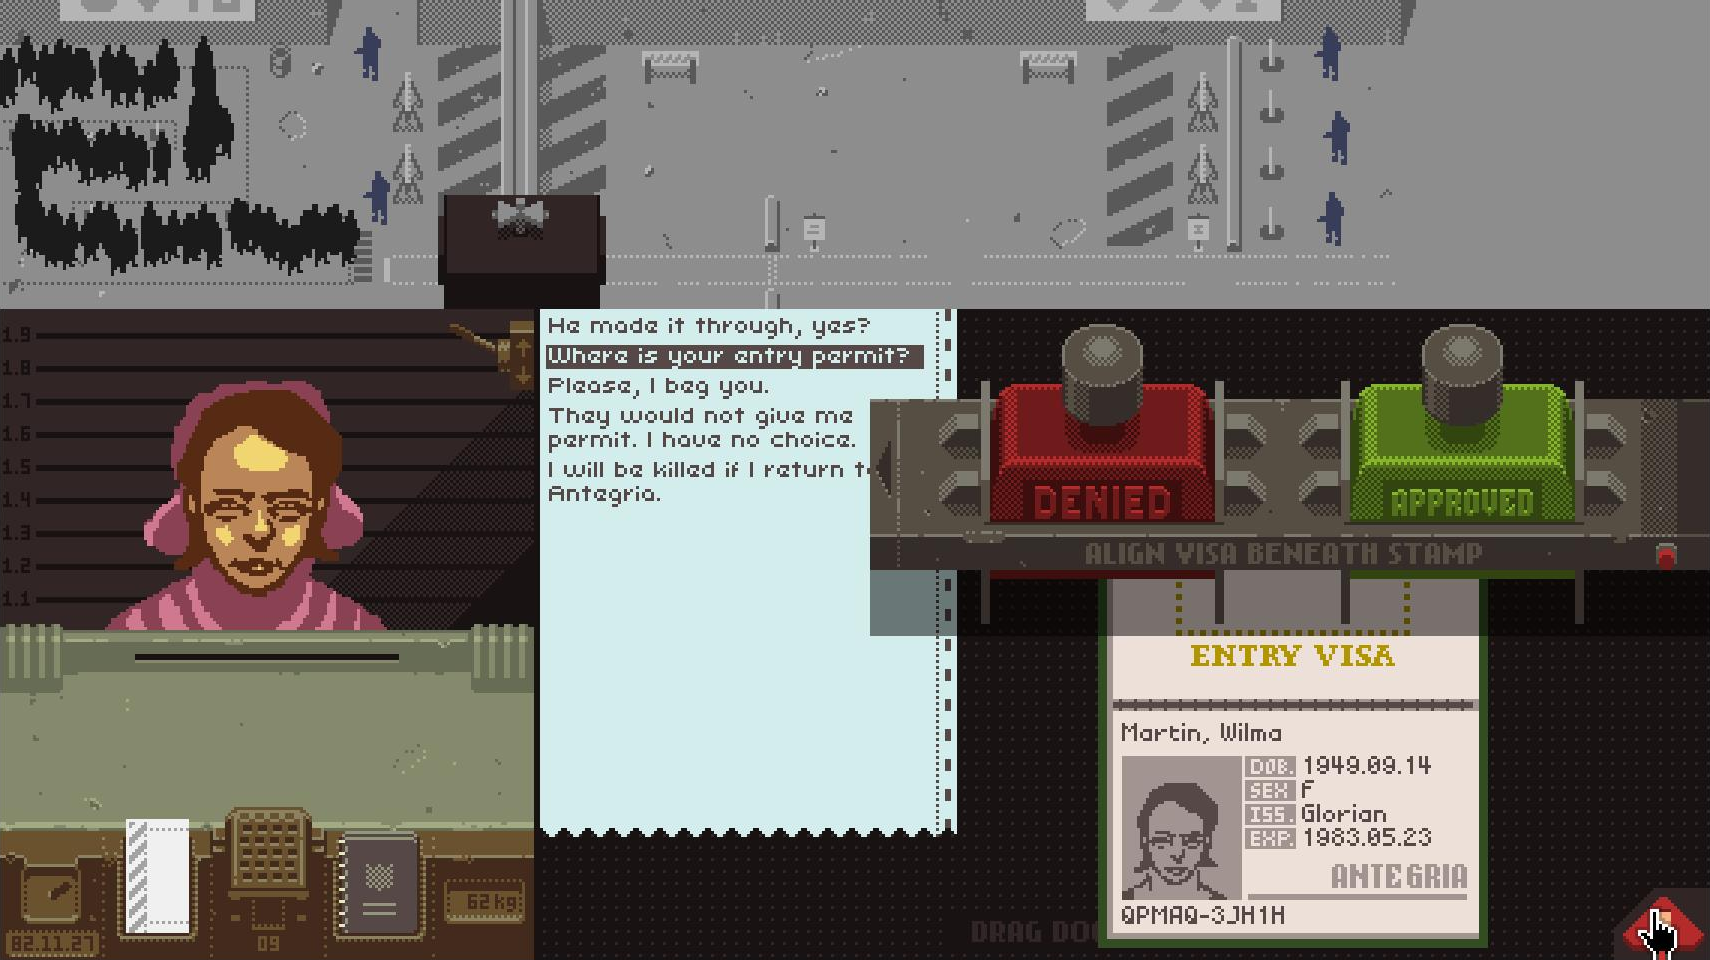
\includegraphics[height=0.3\textheight]{res/papersplease-large.png} \\
  \vspace*{1em}
  \footnotesize
  \begin{tabular}{c c c c c}
    \toprule
    &  \multicolumn{2}{c}{\textit{Doubtful}} & \multicolumn{2}{c}{\textit{Trusting}} \\
    \midrule
    \textbf{Goal} & \textbf{Approve} & \textbf{Deny} & \textbf{Approve} & \textbf{Deny} \\
    \midrule
    \multirow{2}{*}{<treat ethically>} & \textbf{enables}  & \textbf{enables}   & \textbf{enables}  & \textbf{threatens} \\
                                       &                   & \textbf{threatens} & \textbf{advances} & \textbf{hinders}   \\
    \midrule

    <stop cheaters> & \textbf{threatens} & \textbf{enables} & \emph{none} & \emph{none} \\
    \bottomrule
  \end{tabular}
\end{frame}

\begin{frame}{Example: Relative Option Analysis}
  \centering
  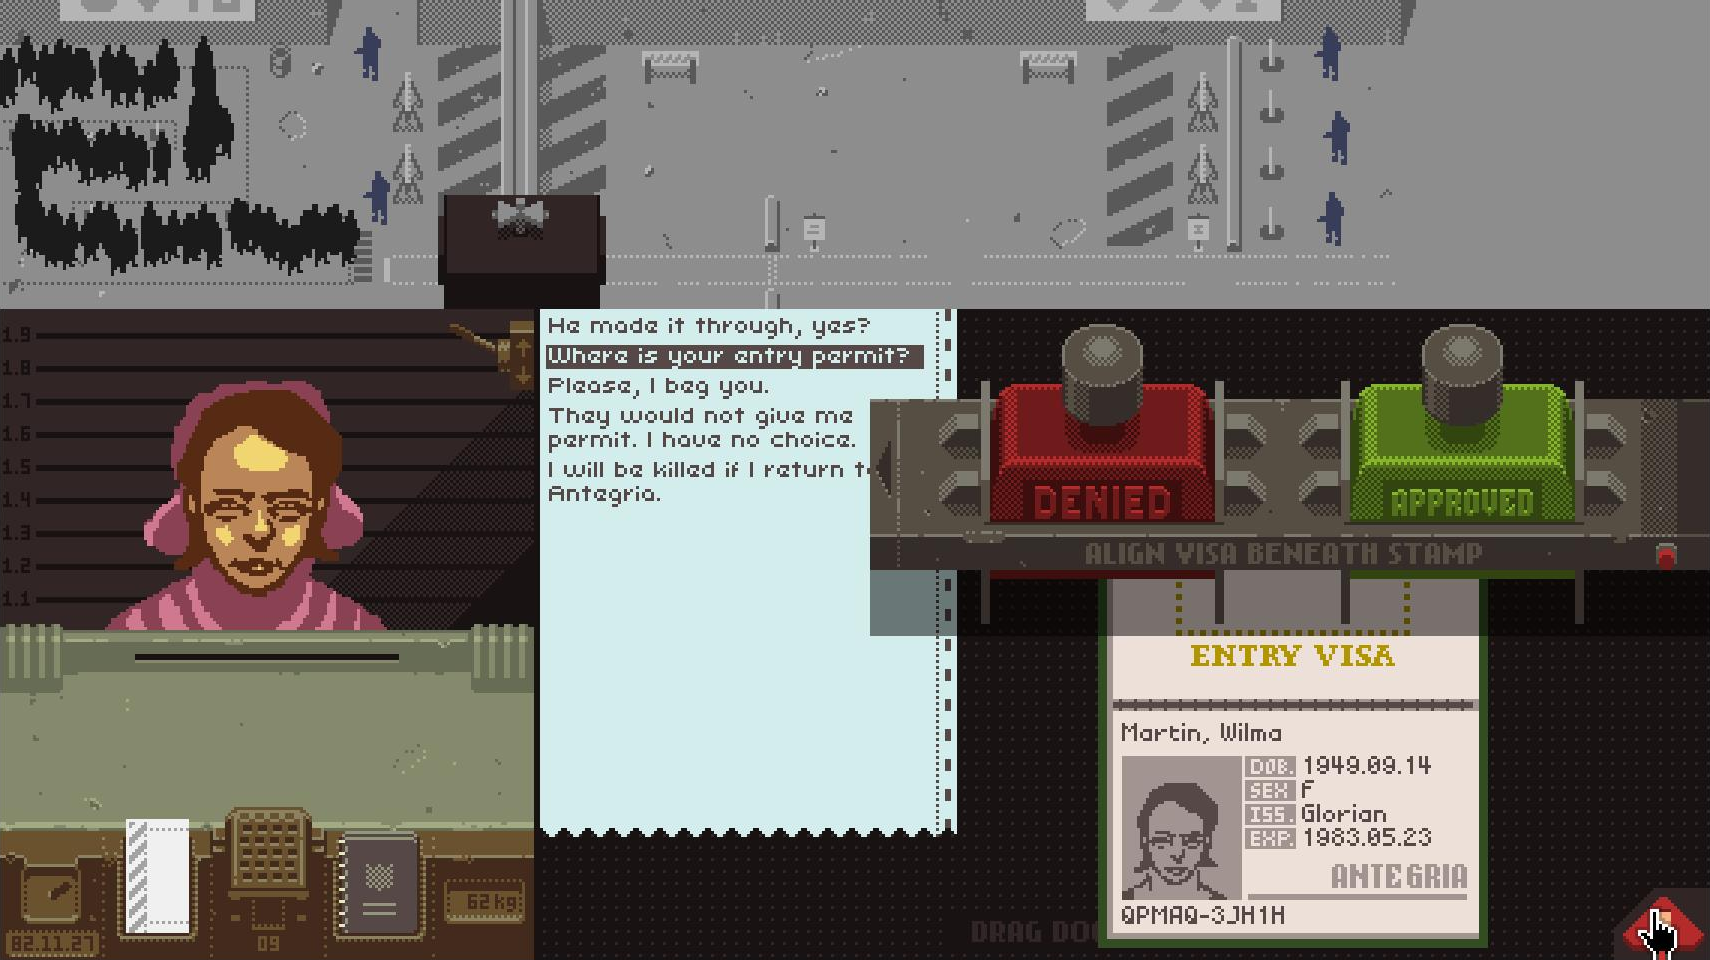
\includegraphics[height=0.3\textheight]{res/papersplease-large.png} \\
  \vspace*{0.5em}
  \footnotesize
  \begin{tabular}{c c c}
    \toprule
    \textbf{Goal} & \textbf{Approve} & \textbf{Deny} \\
    \midrule
    \multirow{3}{*}{<feed your family>} & \textbf{enables} & \textbf{enables} \\
                                        & \textbf{threatens} & \\
                                        & \textbf{hinders} & \textbf{advances} \\
    \midrule

    \multirow{3}{*}{<avoid penalty>} & \textbf{enables} & \textbf{enables} \\
                                     & \textbf{threatens} & \\
                                     & \textbf{hinders} & \textbf{advances} \\
    \midrule

    \multirow{2}{*}{<treat ethically>} & \textbf{enables} & \textbf{threatens} \\
                                       & \textbf{advances} & \textbf{hinders} \\
    \bottomrule
  \end{tabular}
\end{frame}

\begin{frame}{Example: Relative Option Analysis}
  \centering
  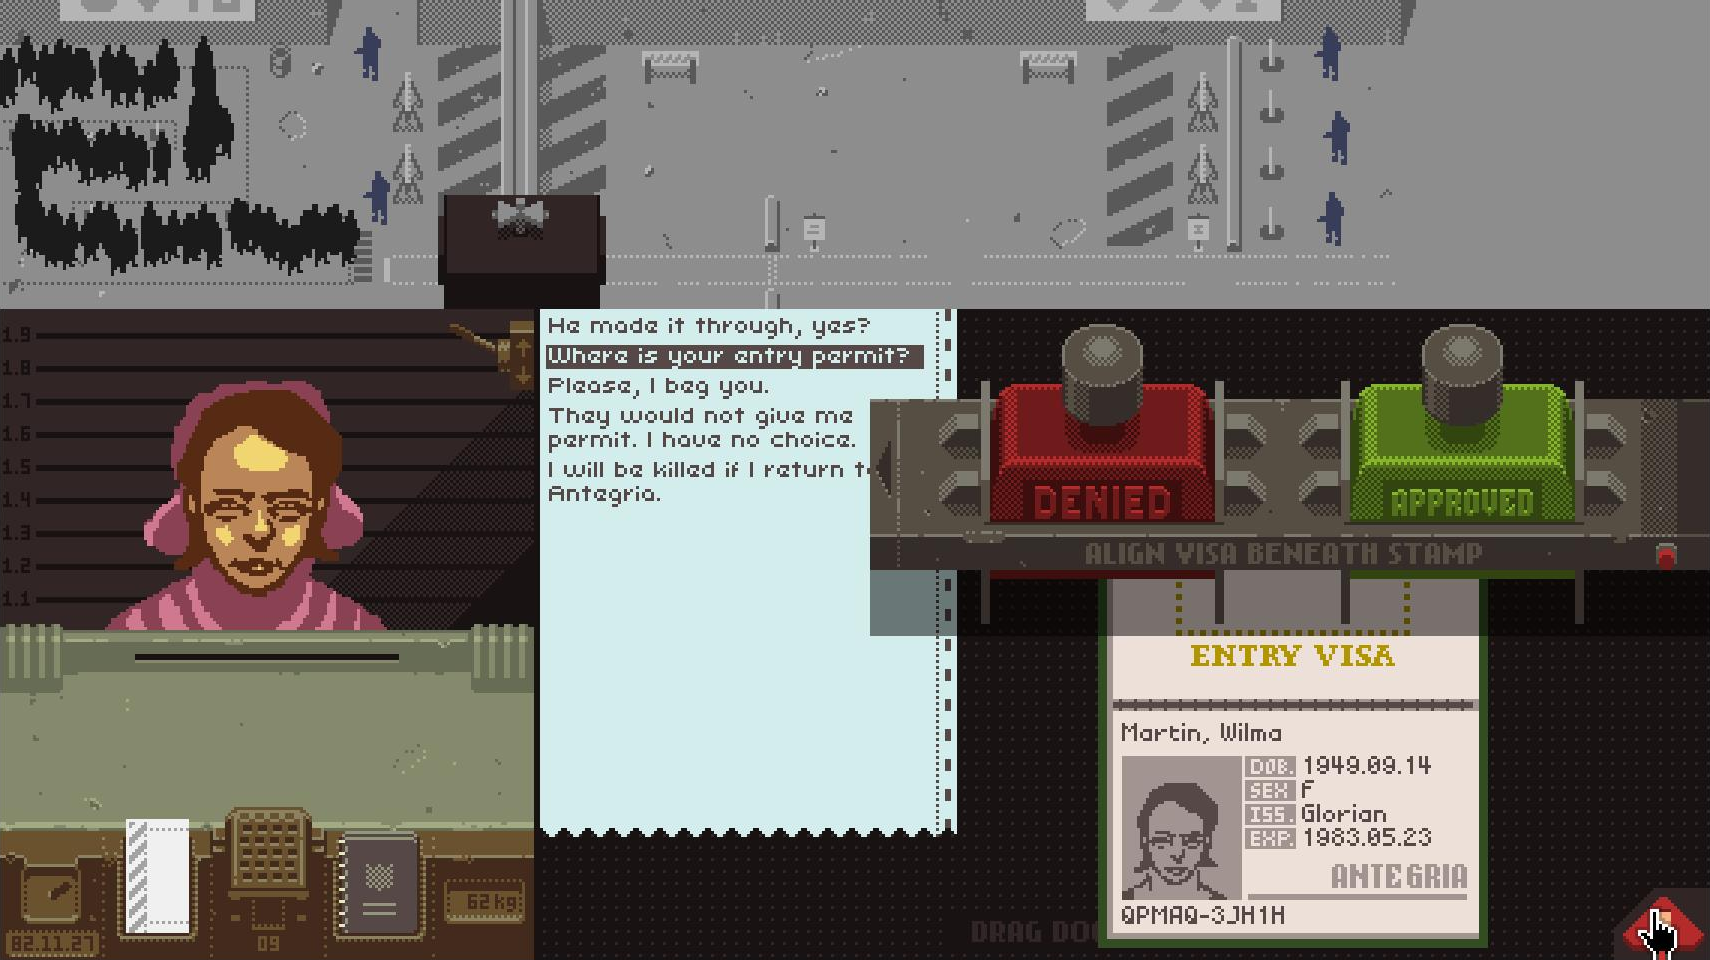
\includegraphics[height=0.3\textheight]{res/papersplease-large.png} \\
  \vspace*{0.5em}
  \footnotesize
  \begin{tabular}{c c c}
    \toprule
    \textbf{Goal} & \textbf{Approve} & \textbf{Deny} \\
    \midrule
    \multirow{3}{*}{<feed your family>} & \textbf{enables} & \textbf{enables} \\
                                        & \textbf{threatens} & \\
                                        & \underline{\textbf{hinders}} & \textbf{advances} \\
    \midrule

    \multirow{3}{*}{<avoid penalty>} & \textbf{enables} & \textbf{enables} \\
                                     & \textbf{threatens} & \\
                                     & \underline{\textbf{hinders}} & \textbf{advances} \\
    \midrule

    \multirow{2}{*}{<treat ethically>} & \textbf{enables} & \textbf{threatens} \\
                                       & \textbf{advances} & \underline{\textbf{hinders}} \\
    \bottomrule
  \end{tabular}
\end{frame}

\begin{frame}{Example: Relative Option Analysis}
  \centering
  \textbf{Dilemma} \\
  \vspace{0.5\baselineskip}
  \raggedright
Exactly two options, each of which \textbf{hinders} one of two different high-priority player goals.
%
The priorities of the goals and the severity of the consequences should be balanced and neither option should \textbf{enable} or \textbf{advance} any goals (even low-priority ones).
\end{frame}

\begin{frame}{Example: Prospective Impression}
  \centering
  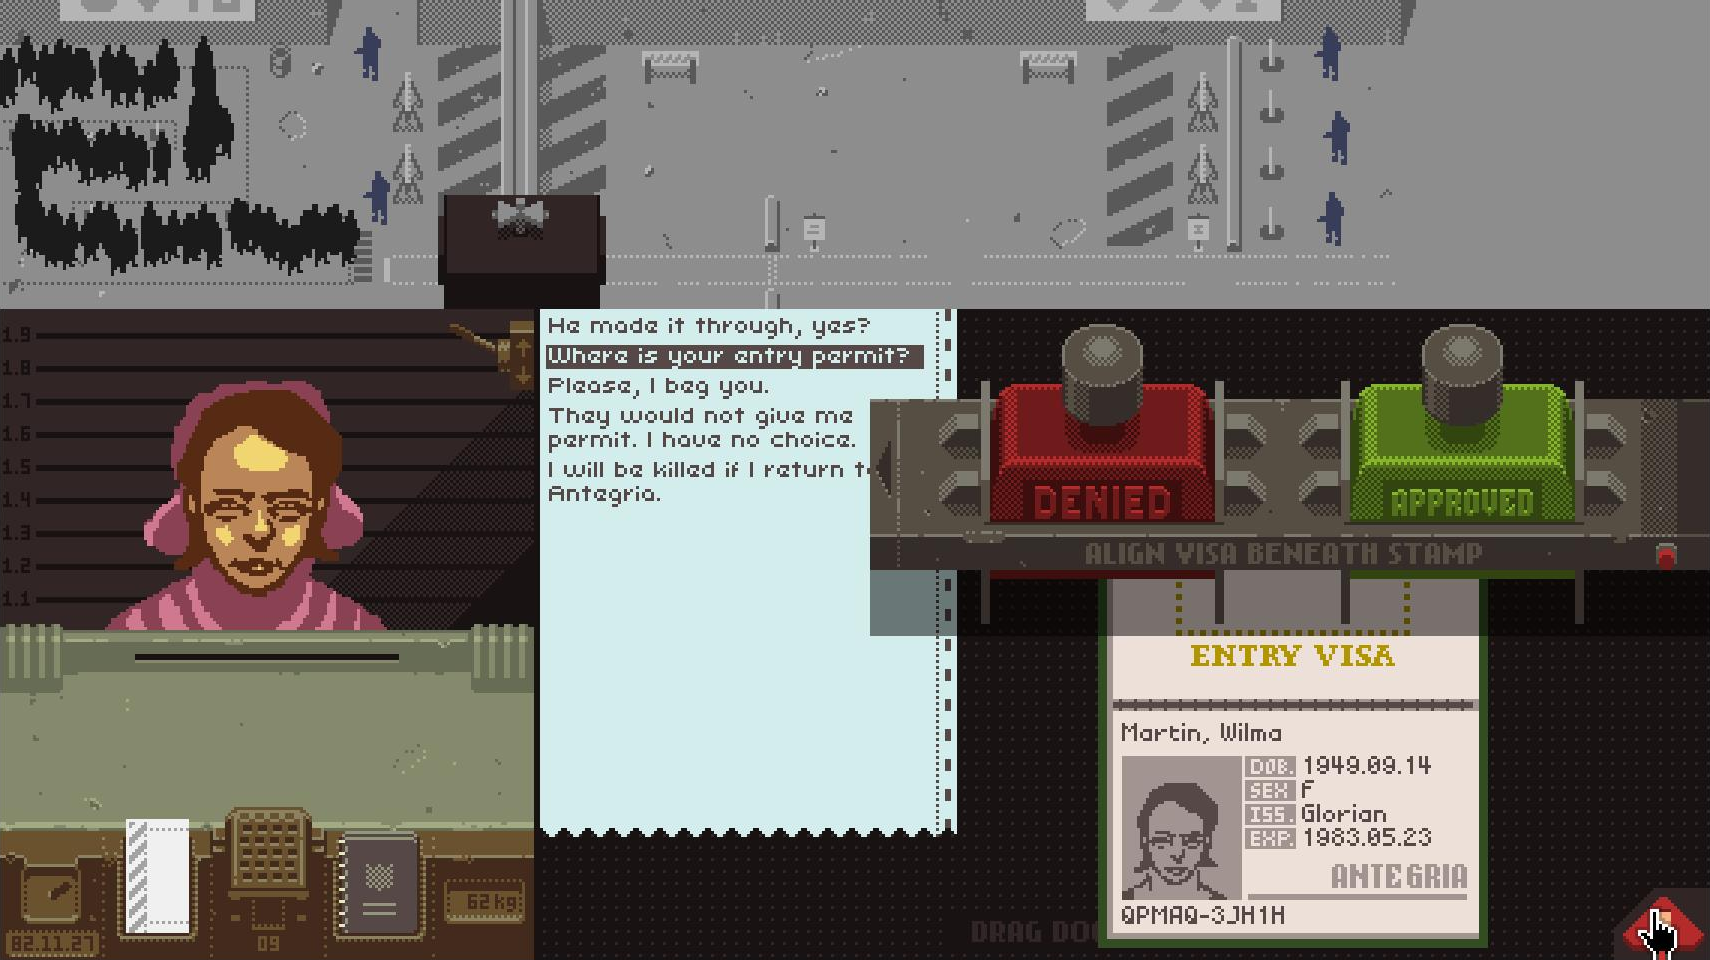
\includegraphics[width=0.9\textwidth]{res/papersplease-large.png} \\
  \vspace{1em}
  \pause
  \textbf{dilemma + doubt = complicity}
\end{frame}

\begin{frame}{5. Outcome Component Analysis}
  \begin{itemize}\addtolength{\itemsep}{0.5\baselineskip}
    \item The impact of each actual outcome component on each player goal is considered.
    \item Major/minor positive/negative labels may be used, or some finer scale of good/bad impacts.
    \item The \emph{suggested} outcome components from the likelihood analysis step may not be \emph{actual}.
    \item There may also be \emph{non-suggested} \emph{actual} outcome components.
    \item In some cases, probability can be folded into severity.
  \end{itemize}
\end{frame}

\begin{frame}{6. Full Outcome Analysis}
  \begin{itemize}\addtolength{\itemsep}{0.5\baselineskip}
    \item Information from goal analysis, likelihood analysis, and outcome component analysis is combined.
    \item Entire outcomes are categorized as \textbf{good}, \textbf{bad}, \textbf{irrelevant} or \textbf{tradeoffs} according to the effects their components have on various goals.
    \item Outcomes are also categorized as \textbf{expected}, \textbf{unexpected}, or \textbf{unpredictable} based on comparing the results of likelihood analysis with the results of outcome component analysis.
    \item These \emph{valence} and \emph{expectedness} values give a wholistic view of the outcome of each option.
  \end{itemize}
\end{frame}

\begin{frame}{7. Retrospective Analysis}
  \begin{itemize}\addtolength{\itemsep}{0.5\baselineskip}
    \item Estimates \textbf{retrospective impressions} using information from relative option analysis and full outcome analysis.
    \item Different options usually have different \textbf{retrospective impressions}.
    \item As with the \textbf{prospective impression} of an entire choice, exemplars such as \textbf{miracle} or \textbf{unfair} anchor the analysis.
  \end{itemize}
  \vfill
  \centering
  \scriptsize (My second experiment tested the \textbf{expected success}, \textbf{expected failure}, \textbf{unfair}, and \textbf{miracle} impressions.)
\end{frame}

\begin{frame}{7. Retrospective Analysis}
\centering
\renewcommand*{\arraystretch}{1.5}
\footnotesize
\hspace*{-1.5em}
\begin{tabular}{p{4.5em}p{12em}p{16.5em}}
\toprule
\textbf{Label} & \textbf{Description} & \textbf{Criteria} \\
\midrule
\textbf{Expected Success} & A predictable outcome that advances player goals. & The option selected \textbf{advances} a player goal without \textbf{hindering} any, and its outcome is both \textbf{predictable} and \textbf{good}. \\
\textbf{Unfair} & An option that seemed good but had unexpected negative consequences. & The selected option must be expected to \textbf{advance} at least one high-priority player goal, while not \textbf{hindering} any. It must also have an \textbf{unexpected} and \textbf{bad} outcome. \\
\textbf{Miracle} & An option that seemed like a lost cause but that unexpectedly turned out well. & The selected option must be expected to \textbf{fail} at least one high-priority goal, while not \textbf{advancing} any. It must have an \textbf{unexpected} and \textbf{good} outcome. \\
\bottomrule
\end{tabular}
\end{frame}

\begin{frame}{Outline}
  \begin{itemize}
    \item Motivation
    \item Inspiration: \skald/ and \problemplanets/
    \item Methodology
    \item Related Work
    \item Theory: Choice Poetics
    \item \textbf{Application: \dunyazad/}
    \item \textbf{Results: Options}
    \item \textbf{Results: Outcomes}
    \item \textbf{Conclusions}
  \end{itemize}
\end{frame}

\begin{frame}{\dunyazad/}
  \begin{itemize}\addtolength{\itemsep}{0.5\baselineskip}
    \item \dunyazad/ is an operationalization of goal-based choice analysis.
    \item Using answer set programming, it solves for choice structures with specified prospective and retrospective impressions.
    \item Imperative code can chain these choices together into an interactive story.
    \item Choice structures are converted into English text and code (HTML or similar).
  \end{itemize}
\end{frame}

\begin{frame}{Constraints}
  \begin{itemize}\addtolength{\itemsep}{0.5\baselineskip}
    \item \textbf{Representational constraints} define the basic elements of choices.
    \item \textbf{Constitutent constraints} define how those elements come together to form choices.
    \item \textbf{Aesthetic constraints} limit the kinds of configurations allowed to those that make sense.
    \item \textbf{Poetic constraints} distinguish between allowed configurations and permit users to request specific impressions.
  \end{itemize}
\end{frame}

\begin{frame}{State Representation}
  \centering
  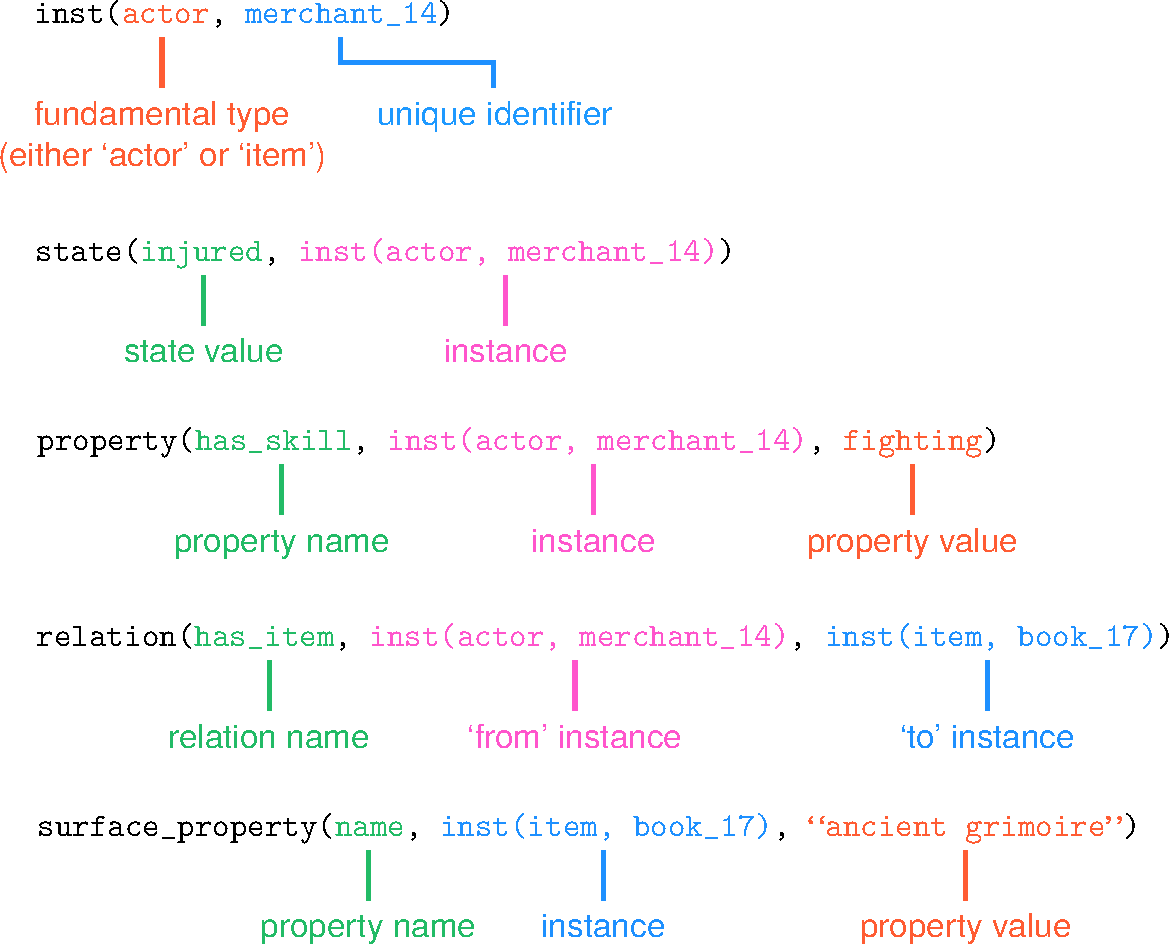
\includegraphics[height=0.8\textheight]{fig/cropped-dunyazad-states.pdf}
\end{frame}

\begin{frame}{State Representation}
  \centering
\fbox{%
\parbox{\textwidth}{
  \small
Scene:\svind\\
\ind ``A merchant carrying some perfume is being threatened by bandits.''\vind\\
Representation:\svind \\
\ind \parbox{0.9\textwidth}{ \tt
\scriptsize
inst(actor,businessperson\_4). \\
inst(actor,tough\_3). \\
inst(item,treasure\_5). \\
property(type,inst(actor,businessperson\_4),merchant). \\
property(type,inst(actor,tough\_3),bandits). \\
property(type,inst(item,treasure\_5),perfume). \\
relation( \\
\ind has\_item, \\
\ind inst(actor,businessperson\_4), \\
\ind inst(item,treasure\_5) \\
). \\
relation( \\
\ind threatening, \\
\ind inst(actor,tough\_3), \\
\ind inst(actor,businessperson\_4) \\
). \\
surface\_property(name,inst(item,treasure\_5),"perfume").
}
}
}
\end{frame}

\begin{frame}{Action Representation}
  \begin{itemize}\addtolength{\itemsep}{0.5\baselineskip}
    \item Each state has one or more options, which lead to other states.
    \item Each option corresponds to an action, with variable pre- and post-conditions.
    \item Effects of an action are split across outcome components, for example \prq{victory}{,} \prq{defeat}{,} and \prq{draw}{} for the \prq{attack}{} action.
    \item Outcome components may be exclusive, and each may have its own preconditions.
    \item At each option, the active outcome components are fixed, and the corresponding state changes are recorded as consequences.
  \end{itemize}
\end{frame}

\begin{frame}{Action Inventory}
\vfill
\centering
\renewcommand*{\arraystretch}{1.5}
\footnotesize
\hspace*{-1.5em}
\begin{tabular}{c c c c}
  \pr{accuse}       & \pr{explain\_innocence} & \pr{play\_song}         & \pr{talk\_down} \\
  \cg{\pr{arrive}*}       & \pr{flee}               & \pr{polymorph}          & \pr{tell\_story} \\
  \pr{attack}       & \pr{gossip}             & \cg{\pr{pursue}*}             & \pr{trade} \\
  \pr{buy\_healing} & \pr{leave}              & \pr{reach\_destination} & \pr{travel\_onwards} \\
  \pr{deny\_blame}  & \pr{pacify}             & \pr{shift\_blame}       & \pr{treat\_injury} \\
  \pr{dispel}       & \pr{pay\_off}           & \pr{steal}
\end{tabular}
\vfill
\normalsize
\dunyazad/'s 23 current actions.
\end{frame}

\begin{frame}{Setups}
  \begin{itemize}\addtolength{\itemsep}{0.5\baselineskip}
    \item \dunyazad/ uses \textbf{setups} to create interesting situations.
    \item Each \textbf{setup} includes some variable parts.
    \item Once \textbf{potentials} are resolved, the characters ``travel onwards'' and a new setup is invoked.
    \item Combined with rules for character motivation, \textbf{potentials} drive the action forward.
  \end{itemize}
\end{frame}

\begin{frame}{Constituent Constraints}
  \begin{itemize}\addtolength{\itemsep}{0.5\baselineskip}
    \item Motivation, relevance, repetition, etc.
    \item Likely outcomes based on character skills and tools.
    \item Common-sense rules (e.g., being incapacitated).
  \end{itemize}
\end{frame}

\begin{frame}{Aesthetic Constraints}
  \begin{itemize}\addtolength{\itemsep}{0.5\baselineskip}
    \item Enforce narrative perspective (second person).
    \item Mandate variety and track boredom.
    \item Exclude undesirable configurations (e.g., trick options).
  \end{itemize}
\end{frame}

\begin{frame}{Poetic Constraints}
  \begin{itemize}\addtolength{\itemsep}{0.5\baselineskip}
    \item Each step of goal-based choice analysis is represented.
    \item Goal analysis consists of hand-specified player goals:
    \begin{itemize}\addtolength{\itemsep}{0.5\baselineskip}
      \vspace{0.5\baselineskip}
      \item {[high]}\prq{preserve\_health}{}
      \item {[high]}\prq{avoid\_threats\_to}{}
      \item {[high]}\prq{avoid\_accusations}{}
      \item {[high]}\prq{preserve\_original\_form}{}
      \item {[high]}\prq{reclaim\_property}{}
      \item {[low]}\prq{as\_intended}{}
      \item {[low]}\prq{have\_tool\_for}{}
    \end{itemize}
    \item Skill links are used to determine likelihoods.
  \end{itemize}
\end{frame}

\begin{frame}{Output Example}
  \itshape
You come to a tavern and decide to rest for a while.
%
A merchant is bored and a noble is bored and an innkeeper seems knowledgeable.
%
What do you do?
\begin{enumerate}
\item You play a song for the noble \\
  (You have skill: musician. You have no tool for music).
\item You gossip with the innkeeper \\
  (You are missing skill: negotiation).
\item You play a song for the merchant \\
  (You have skill: musician. You have no tool for music).
\end{enumerate}
\end{frame}

\begin{frame}{Outline}
  \begin{itemize}
    \item Motivation
    \item Inspiration: \skald/ and \problemplanets/
    \item Methodology
    \item Related Work
    \item Theory: Choice Poetics
    \item Application: \dunyazad/
    \item \textbf{Results: Options}
    \item \textbf{Results: Outcomes}
    \item \textbf{Conclusions}
  \end{itemize}
\end{frame}

\begin{frame}{Option Experiment}
  \begin{itemize}\addtolength{\itemsep}{0.5\baselineskip}
    \item An online experiment using choices created by \dunyazad/.
    \item Participants read a choice and then answered questions.
    \begin{itemize}\addtolength{\itemsep}{0.5\baselineskip}
      \vspace{0.5\baselineskip}
      \item 90 Amazon Mechanical Turk workers (+6 rejected).
      \item \$0.50 per task (one per worker).
      \item Median response time was 4:40.
      \item Two questions were used to filter responses and incompletes were removed, leaving 79 valid responses.
      \item The rest of the survey consisted of seven 5-point Likert items.
    \end{itemize}
  \end{itemize}
\end{frame}

\begin{frame}{Experiment Design}
  \begin{itemize}\addtolength{\itemsep}{0.5\baselineskip}
    \item The question: \emph{``Is \dunyazad/ successfully creating the desired prospective impressions?''}
    \item The \textbf{relaxed}, \textbf{obvious}, and \textbf{dilemma} impressions were used because they cover positive/negative, balanced/imbalanced, and high-/low-stakes options.
    \item \dunyazad/ generated three choices per condition and ten participants saw each choice ($3 \times 3 \times 10 = 90$).
  \end{itemize}
\end{frame}

\begin{frame}{Survey Questions}
  \itshape
  \begin{enumerate}\addtolength{\itemsep}{0.5\baselineskip}
    \item ``There are no bad options at this choice.''
    \item ``There is a clear best option at this choice.''
    \item ``The stakes for this choice are low.''
    \item ``There are no good options at this choice.''
    \item ``All of the options at this choice are about equally promising.''
    \item ``There are options at this choice.'' (This is a trick question to test whether you’re paying attention. Please simply indicate that you are in complete disagreement.)
    \item ``This is a difficult choice to make.''
    \item ``This choice feels like it will have important consequences.''
  \end{enumerate}
\end{frame}

\begin{frame}{Results}
  \centering
  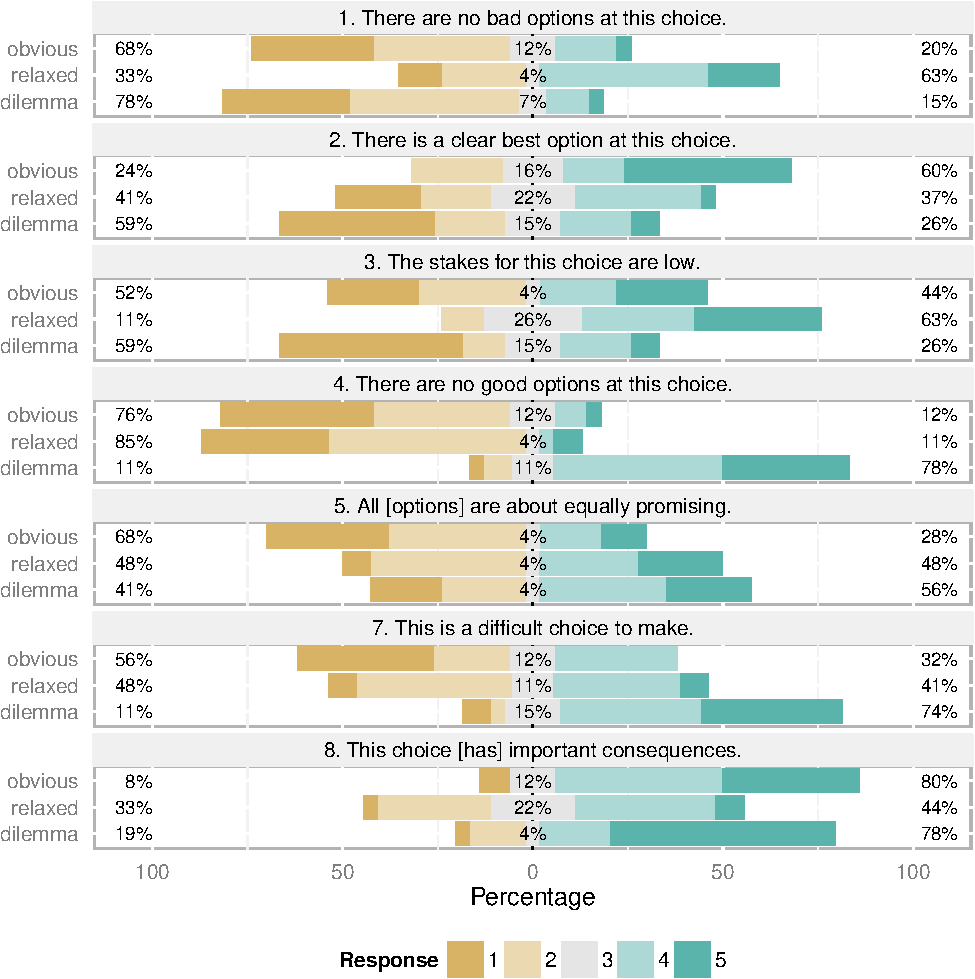
\includegraphics[height=0.85\textheight]{fig/combined-report-cropped.pdf}
\end{frame}

\begin{frame}{Outline}
  \begin{itemize}
    \item Motivation
    \item Inspiration: \skald/ and \problemplanets/
    \item Methodology
    \item Related Work
    \item Theory: Choice Poetics
    \item Application: \dunyazad/
    \item Results: Options
    \item \textbf{Results: Outcomes}
    \item \textbf{Conclusions}
  \end{itemize}
\end{frame}

\begin{frame}{Outline}
  \begin{itemize}
    \item Motivation
    \item Inspiration: \skald/ and \problemplanets/
    \item Methodology
    \item Related Work
    \item Theory: Choice Poetics
    \item Application: \dunyazad/
    \item Results: Options
    \item Results: Outcomes
    \item \textbf{Conclusions}
  \end{itemize}
\end{frame}

\begin{frame}{Questions?}
  \begin{itemize}
    \item Motivation
    \item Inspiration: \skald/ and \problemplanets/
    \item Methodology
    \item Related Work
    \item Theory: Choice Poetics
    \item Application: \dunyazad/
    \item Results: Options
    \item Results: Outcomes
    \item Conclusions
  \end{itemize}
\end{frame}

%\begin{frame}{Na\"{i}ve Approach}
%It was the spring of 1089, and a knight named Lancelot returned to Camelot from elsewhere. Lancelot was hot tempered. Once, Lancelot had lost a joust. Because he was hot tempered, Lancelot wanted to destroy his sword. Lancelot struck his sword. His sword was destroyed.
%\end{frame}
%
%\begin{frame}{Na\"{i}ve Approach}
%\begin{center}
%  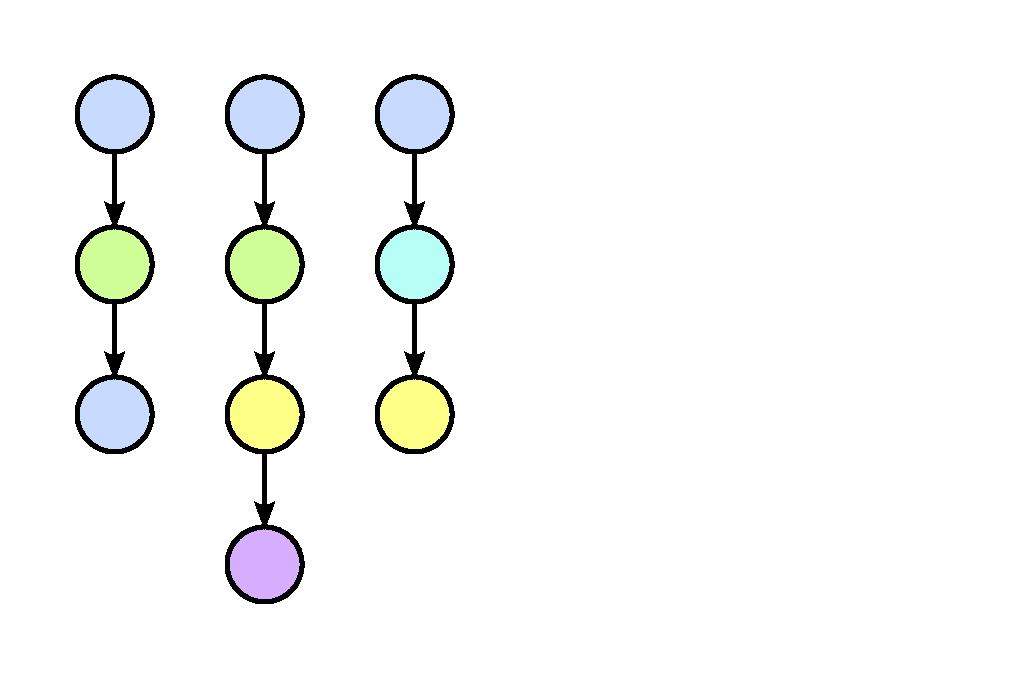
\includegraphics[width=0.9\textwidth]{res/naive-cyoa-linear.pdf}
%\end{center}
%\end{frame}
%
%\begin{frame}{Na\"{i}ve Approach}
%\begin{center}
%  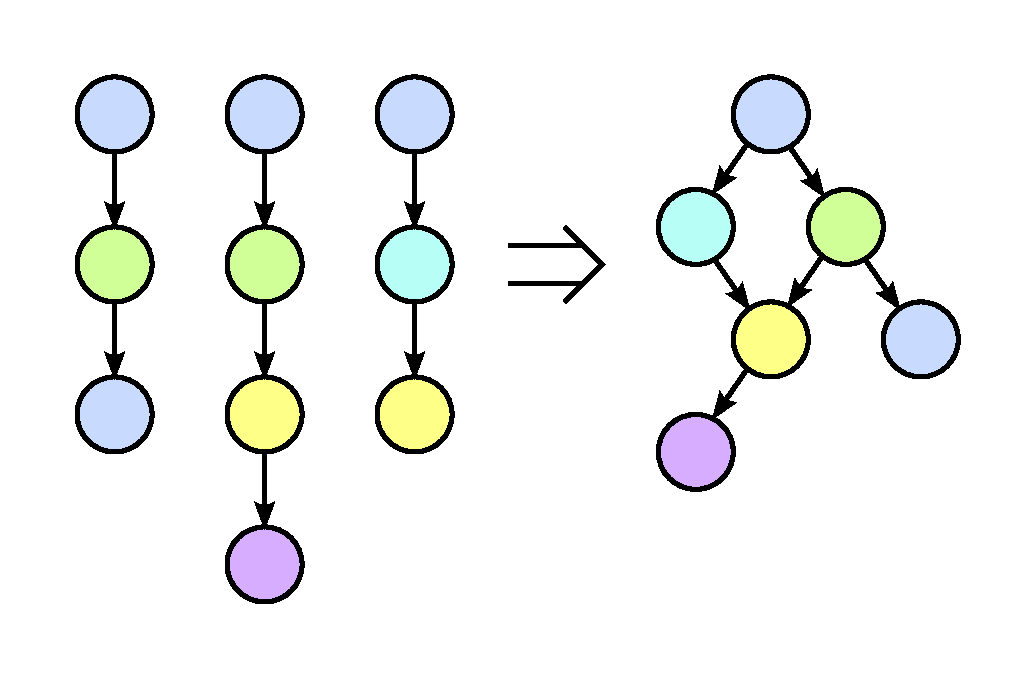
\includegraphics[width=0.9\textwidth]{res/naive-cyoa.pdf}
%\end{center}
%\end{frame}
%
%\begin{frame}{The Problem}
%\begin{itemize}
%  \item Where do you put the branches?
%  \item How many options should each branch have?
%  \item What outcomes should the different branches have?
%\end{itemize}
%%\pause
%%\begin{center}
%%How do choices affect the narrative?
%%\end{center}
%\end{frame}
%
%\begin{frame}{The Problem}
%\begin{itemize}
%  \item How do choices affect a narrative?
%\end{itemize}
%\end{frame}
%
%\begin{frame}{The Solution}
%  \itshape
%  ``By reasoning deliberately about choices \textbf{using a theory of choice poetics}, a generative narrative system can construct fixed-form branching narratives that give the player a feeling of agency which persists even when different branches of those narratives are explored.''
%\end{frame}
%
%\begin{frame}{The System}
%  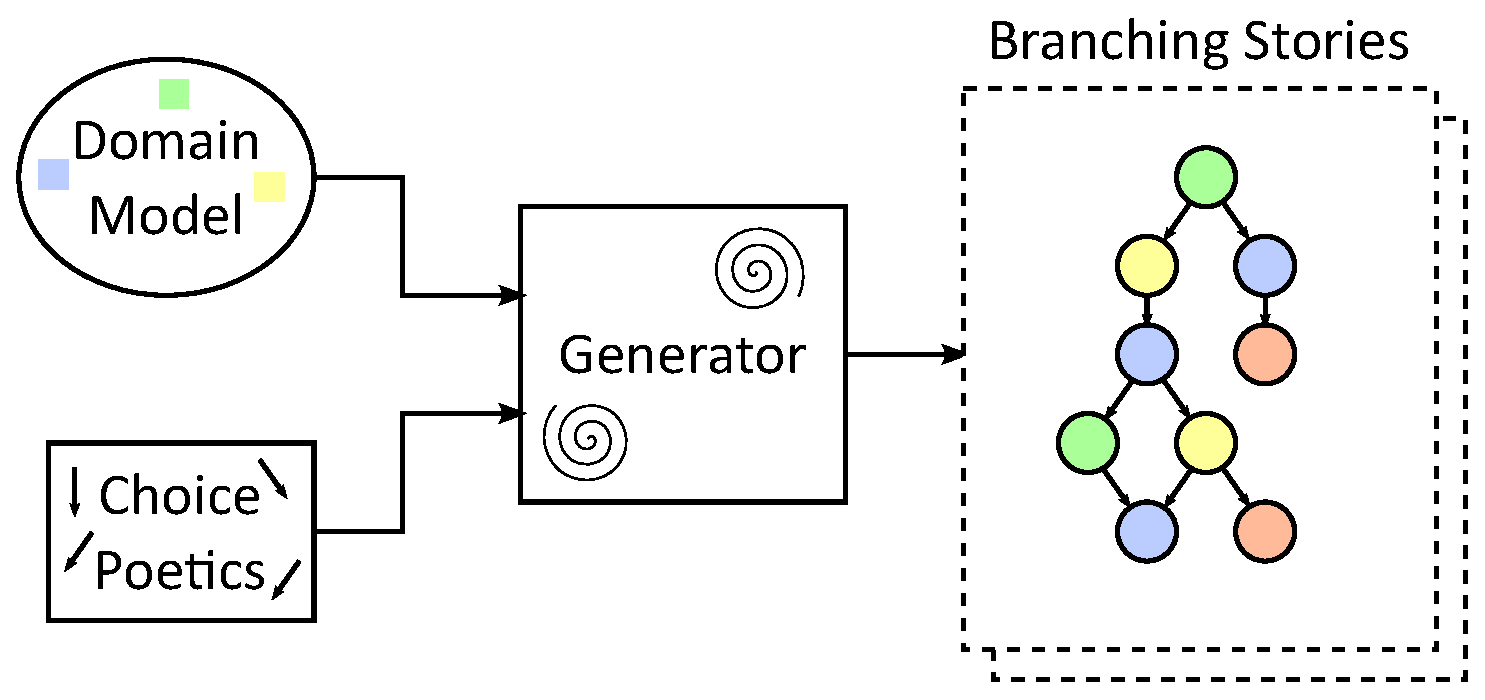
\includegraphics[width=0.9\textwidth]{res/high-level-architecture.eps}
%\end{frame}
%
%\begin{frame}{Outline}
%  \begin{itemize}
%    \item Related work
%    \item Choice poetics
%    \begin{itemize}
%      \item Modes of engagement
%      \item Choice idioms
%      \item Dimensions of player experience
%    \end{itemize}
%    \item More related work
%    \item Technical approach
%    \begin{itemize}
%      \item Story Domain
%      \item Generating narrative
%      \item Generating choices
%    \end{itemize}
%    \item Evaluation
%    \begin{itemize}
%      \item Empirical
%      \item Critical
%    \end{itemize}
%  \end{itemize}
%\end{frame}
%
%\begin{frame}{Outline}
%  \begin{itemize}
%    \item \textbf{Related work}
%    \item Choice poetics
%    \begin{itemize}
%      \item Modes of engagement
%      \item Choice idioms
%      \item Dimensions of player experience
%    \end{itemize}
%    \item More related work
%    \item Technical approach
%    \begin{itemize}
%      \item Story Domain
%      \item Generating narrative
%      \item Generating choices
%    \end{itemize}
%    \item Evaluation
%    \begin{itemize}
%      \item Empirical
%      \item Critical
%    \end{itemize}
%  \end{itemize}
%\end{frame}
%
%\begin{frame}{Narrative Theory: Poetics}
%  \begin{tabular}{C{0.45\textwidth} C{0.45\textwidth}}
%    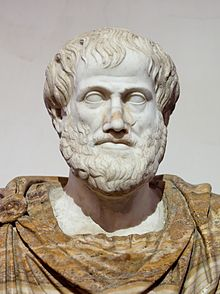
\includegraphics[height=0.3\textwidth]{res/aristotle.jpg} &
%    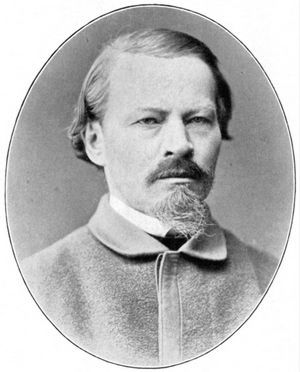
\includegraphics[height=0.3\textwidth]{res/freytag.jpg} \\
%    Aristotle & Gustav Freytag \\
%    \work{Poetics} & \work{Technique of the Drama} \\
%    circa 335 B.C. & 1894 \\
%  \end{tabular}
%\end{frame}
%
%\begin{frame}{Narrative Theory: Structuralism}
%  \begin{tabular}{C{0.45\textwidth} C{0.45\textwidth}}
%    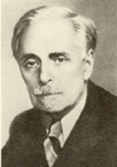
\includegraphics[height=0.3\textwidth]{res/propp.jpg} &
%    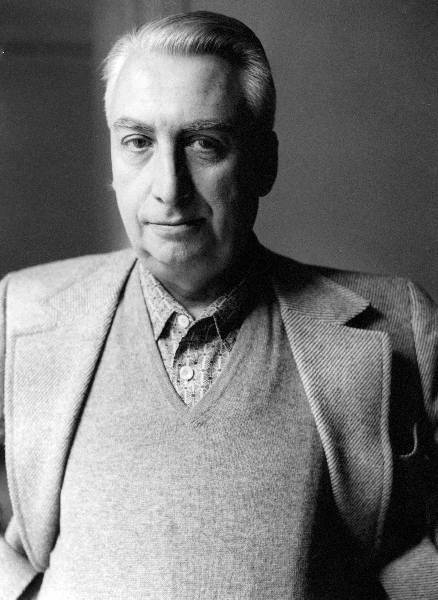
\includegraphics[height=0.3\textwidth]{res/barthes.jpg} \\
%    Vladimir Propp & Roland Barthes \\
%    \work{Morphology of the Folktale} & \work{An Introduction to the Structural Analysis of Narrative} \\
%    1928 & 1975 \\
%  \end{tabular}
%\end{frame}
%
%\begin{frame}{Narrative Theory: Effects}
%  \begin{tabular}{C{0.45\textwidth} C{0.45\textwidth}}
%    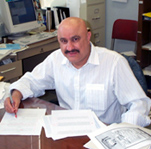
\includegraphics[height=0.3\textwidth]{res/iran-nejad.jpg} &
%    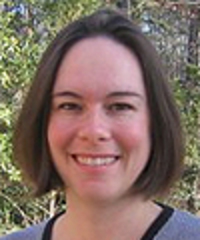
\includegraphics[height=0.3\textwidth]{res/green.jpg} \hspace*{2pt}
%    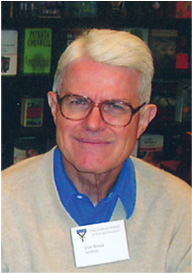
\includegraphics[height=0.3\textwidth]{res/brock.jpg} \\
%    Asghar Iran-Nejad & Melanie Green \& Timothy Brock \\
%    \work{Cognitive and Affective Causes of Interest and Liking} & \work{The Role of Transportation in the Persuasiveness of Public Narratives} \\
%    1987 & 2000 \\
%  \end{tabular}
%\end{frame}
%
%\begin{frame}{Narrative Theory: Hypertext}
%  \begin{tabular}{C{0.3\textwidth} C{0.3\textwidth} C{0.3\textwidth}}
%    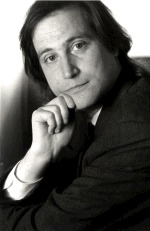
\includegraphics[height=0.3\textwidth]{res/bernstein.jpg} &
%    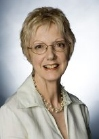
\includegraphics[height=0.3\textwidth]{res/morgan.jpg} &
%    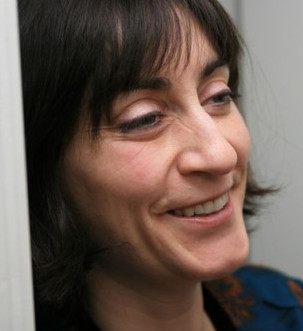
\includegraphics[height=0.3\textwidth]{res/tosca.jpg} \\
%    Mark Bernstein & Wendy Morgan & Susana Tosca\\
%    \work{Patterns of Hypertext} & \work{Heterotopics, Towards a Grammar of Hyperlinks} & \work{A Pragmatics of Links} \\
%    1998 & 1999 & 2000 \\
%  \end{tabular}
%\end{frame}
%
%\begin{frame}{Meaning in Games: Procedural Rhetoric}
%  \begin{tabular}{C{0.45\textwidth} C{0.45\textwidth}}
%    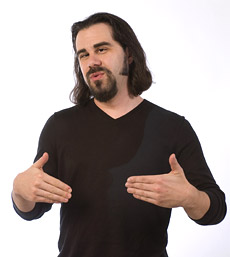
\includegraphics[height=0.3\textwidth]{res/bogost.jpg} &
%    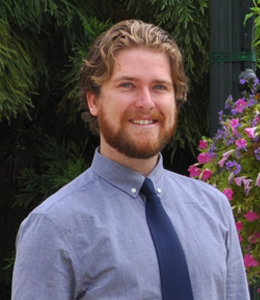
\includegraphics[height=0.3\textwidth]{res/treanor.png} \\
%    Ian Bogost & Mike Treanor \\
%    \work{Persuasive Games} & \work{Investigating Procedural Expression and Interpretation in Videogames} \\
%    2007 & 2013 \\
%  \end{tabular}
%\end{frame}
%
%\begin{frame}{Meaning in Games: Operational Logics \& Agency}
%  \begin{table}[h]
%  \hspace*{-2em}
%  \centering
%  \begin{tabular}{C{0.5\textwidth} C{0.5\textwidth}}
%    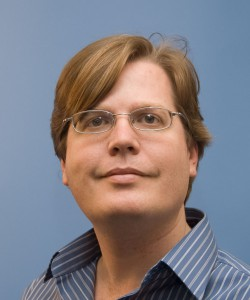
\includegraphics[height=0.3\textwidth]{res/wardrip-fruin.jpg} \hspace*{2pt}
%    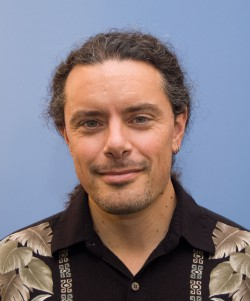
\includegraphics[height=0.3\textwidth]{res/mateas.jpg} &
%    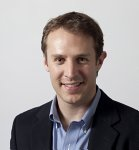
\includegraphics[height=0.28\textwidth]{res/dow.jpg} \hspace*{2pt}
%    
\includegraphics[height=0.28\textwidth]{res/sali.jpg} \\
%    Noah Wardrip-Fruin \& Michael Mateas & \ldots \& Steven Dow \& Serdar Sali \\
%    \work{Defining Operational Logics} & \work{Agency Reconsidered} \\
%    2009 & 2009
%  \end{tabular}
%  \end{table}
%\end{frame}
%
%\begin{frame}{Meaning in Games: Agency}
%  \begin{table}[h]
%  \centering
%  \begin{tabular}{C{0.45\textwidth} C{0.5\textwidth}}
%    \includegraphics[height=0.3\textwidth]{res/laurel.jpg} &
%    \includegraphics[height=0.3\textwidth]{res/murray.jpg} \\
%    Brenda Laurel & Janet Murray\\
%    \work{Toward the Design of a Computer-Based Interactive Fantasy System} &
%    \work{Hamlet on the Holodeck: The Future of Narrative in Cyberspace} \\
%    1986 & 1997
%  \end{tabular}
%  \end{table}
%\end{frame}
%
%\begin{frame}{Critique and Practice}
%  \begin{quote}
%    \slshape
%  This is not your typical brain-teasing adventure game -- it's a character-builder, a choose-your-own adventure where you don't just make decisions, you determine how your character feels about them and how they may affect those around him.
%  \end{quote}
%  \attrib{Matt Buckley, online review of \work{The Wolf Among Us}\footnote{\tiny \url{http://gamingtrend.com/2013/10/24/episode-one-imbues-faith-wolf-among-us/}}}
%\end{frame}
%
%\begin{frame}{Critique and Practice}
%  From the Choice of Games game design blog cateogry\footnote{\url{http://www.choiceofgames.com/category/blog/game-design/}}:
%  \begin{itemize}
%    \item 5 Rules for Writing Interesting Choices in Multiple-Choice Games
%    \item Make a ``Choice of'' Game Your Own: Authorial Intent in IF
%    \item By the Numbers: How to Write a Long Interactive Novel That Doesn’t Suck
%    \item 4 Common Mistakes in Interactive Novels
%  \end{itemize}
%\end{frame}
%
%\begin{frame}{Outline}
%  \begin{itemize}
%    \item Related work
%    \item \textbf{Choice poetics}
%    \begin{itemize}
%      \item Modes of engagement
%      \item Choice idioms
%      \item Dimensions of player experience
%    \end{itemize}
%    \item More related work
%    \item Technical approach
%    \begin{itemize}
%      \item Story Domain
%      \item Generating narrative
%      \item Generating choices
%    \end{itemize}
%    \item Evaluation
%    \begin{itemize}
%      \item Empirical
%      \item Critical
%    \end{itemize}
%  \end{itemize}
%\end{frame}
%
%\begin{frame}{Choice Poetics}
%  \includegraphics[width=\textwidth]{res/two-roads.jpg}
%\end{frame}
%
%\begin{frame}{Choice Poetics}
%  Choices consist of:
%  \begin{itemize}
%    \item Framing
%    \item Options
%    \item Outcomes
%  \end{itemize}
%\end{frame}
%
%\begin{frame}{Choice Poetics}
%  Choices consist of:
%  \begin{itemize}
%    \item Framing--how the choice is presented.
%    \item Options
%    \item Outcomes
%  \end{itemize}
%\end{frame}
%
%\begin{frame}{Choice Poetics}
%  Choices consist of:
%  \begin{itemize}
%    \item Framing--how the choice is presented.
%    \item Options--the alternatives available to the player.
%    \item Outcomes
%  \end{itemize}
%\end{frame}
%
%\begin{frame}{Choice Poetics}
%  Choices consist of:
%  \begin{itemize}
%    \item Framing--how the choice is presented.
%    \item Options--the alternatives available to the player.
%    \item Outcomes--what happens afterwards.
%  \end{itemize}
%\end{frame}
%
%\begin{frame}{Choice Poetics}
%  \includegraphics[width=\textwidth]{res/two-roads.jpg}
%\end{frame}
%
%\begin{frame}{Choice Poetics: Overview}
%  \begin{itemize} 
%    \item Modes of Engagement
%    \item Choice Idioms
%    \item Dimensions of Experience
%  \end{itemize} 
%\end{frame}
%
%\begin{frame}{Choice Poetics: Overview}
%  \begin{itemize} 
%    \item Modes of Engagement--How players approach choices
%    \item Choice Idioms
%    \item Dimensions of Experience
%  \end{itemize} 
%\end{frame}
%
%\begin{frame}{Choice Poetics: Overview}
%  \begin{itemize} 
%    \item Modes of Engagement--How players approach choices
%    \item Choice Idioms--Specific choice structures and their effects
%    \item Dimensions of Experience
%  \end{itemize} 
%\end{frame}
%
%\begin{frame}{Choice Poetics: Overview}
%  \begin{itemize} 
%    \item Modes of Engagement--How players approach choices
%    \item Choice Idioms--Specific choice structures and their effects
%    \item Dimensions of Experience--Things that choice structures affect
%  \end{itemize} 
%\end{frame}
%
%\begin{frame}{Modes of Engagement}
%  \includegraphics[width=\textwidth]{res/scan-book.jpg}
%\end{frame}
%
%\begin{frame}{Modes of Engagement}
%  \begin{itemize}
%    \item Avatar play
%    \item Role play
%    \item Power play
%    \item Exploratory play
%    \item Analytical play
%    \item Critical play
%    \item etc.
%  \end{itemize}
%\end{frame}
%
%\begin{frame}{Modes of Engagement: Avatar Play}
%  \includegraphics[width=\textwidth]{res/avatar-play.jpg}
%\end{frame}
%
%\begin{frame}{Modes of Engagement: Role Play}
%  \includegraphics[width=\textwidth]{res/renfaire.jpg}
%\end{frame}
%
%\begin{frame}{Modes of Engagement: Power Play}
%  \begin{center}
%    \includegraphics[height=0.7\textheight]{res/timmy.jpg}
%  \end{center}
%\end{frame}
%
%\begin{frame}{Modes of Engagement: Exploratory Play}
%  \begin{center}
%    \includegraphics[height=0.7\textheight]{res/exploratory-play.jpg}
%  \end{center}
%\end{frame}
%
%\begin{frame}{Modes of Engagement: Analytical Play}
%  \begin{center}
%    \includegraphics[height=0.8\textheight]{res/chimneyrock.png}
%  \end{center}
%\end{frame}
%
%\begin{frame}{Modes of Engagement: Critical Play}
%  \begin{center}
%    \includegraphics[height=0.8\textheight]{res/alice-in-park.jpg}
%  \end{center}
%\end{frame}
%
%\begin{frame}{Modes of Engagement: Example}
%  \includegraphics[width=\textwidth]{res/me-choice-brighter.png}
%\end{frame}
%
%\begin{frame}{Choice Idioms}
%  \begin{itemize}
%    \item Dilemma
%    \item Flavor choice
%    \item Blind choice
%    \item etc.
%  \end{itemize}
%\end{frame}
%
%\begin{frame}{Choice Idioms: (Di)lemma}
%  \includegraphics[width=\textwidth]{res/starter-pokemon.png}
%\end{frame}
%
%\begin{frame}{Choice Idioms: Flavor Choice}
%  \includegraphics[width=\textwidth]{res/da-customization.jpg}
%\end{frame}
%
%\begin{frame}{Choice Idioms: Blind Choice}
%  \includegraphics[width=\textwidth]{res/megaman2-difficulty.png}
%\end{frame}
%
%\begin{frame}{Dimensions of Experience}
%  \begin{itemize}
%    \item Agency
%    \item Absorption
%    \item Regret
%    \item etc.
%  \end{itemize}
%\end{frame}
%
%\begin{frame}{Dimensions of Experience: Agency}
%  \includegraphics[width=\textwidth]{res/doom-screenshot.jpg}
%\end{frame}
%
%\begin{frame}{Dimensions of Experience: Absorption}
%  \includegraphics[width=\textwidth]{res/absorbed-player.jpg}
%\end{frame}
%
%\begin{frame}{Dimensions of Experience: Regret}
%  \includegraphics[width=\textwidth]{res/twd-regret.jpg}
%\end{frame}
%
%\begin{frame}{Choice Poetics}
%  \color{black} $\rightarrow$ A framework for understanding the narrative effects of choices. \\
%  \pause
%  \begin{center}
%  (this work is only an outline)
%  \end{center}
%\end{frame}
%
%\begin{frame}{Outline}
%  \begin{itemize}
%    \item Related work
%    \item Choice poetics
%    \begin{itemize}
%      \item Modes of engagement
%      \item Choice idioms
%      \item Dimensions of player experience
%    \end{itemize}
%  \item \textbf{More related work}
%    \item Technical approach
%    \begin{itemize}
%      \item Story Domain
%      \item Generating narrative
%      \item Generating choices
%    \end{itemize}
%    \item Evaluation
%    \begin{itemize}
%      \item Empirical
%      \item Critical
%    \end{itemize}
%  \end{itemize}
%\end{frame}
%
%%\begin{frame}{Computational Narrative: History}
%%  \begin{itemize}
%%    \item Klein 1971
%%    \item Meehan 1976
%%    \item Dehn 1981
%%    \item Lebowitz 1984
%%  \end{itemize}
%%\end{frame}
%%
%%\begin{frame}{Computational Narrative: History}
%%  \begin{itemize}
%%    \item Klein 1971--Monte Carlo storytelling
%%    \item Meehan 1976
%%    \item Dehn 1981
%%    \item Lebowitz 1984
%%  \end{itemize}
%%\end{frame}
%%
%%\begin{frame}{Computational Narrative: History}
%%  \begin{itemize}
%%    \item Klein 1971--Monte Carlo storytelling
%%    \item Meehan 1976--recursive character plans
%%    \item Dehn 1981
%%    \item Lebowitz 1984
%%  \end{itemize}
%%\end{frame}
%%
%%\begin{frame}{Computational Narrative: History}
%%  \begin{itemize}
%%    \item Klein 1971--Monte Carlo storytelling
%%    \item Meehan 1976--recursive character plans
%%    \item Dehn 1981--author-level planning
%%    \item Lebowitz 1984
%%  \end{itemize}
%%\end{frame}
%%
%%\begin{frame}{Computational Narrative: History}
%%  \begin{itemize}
%%    \item Klein 1971--Monte Carlo storytelling
%%    \item Meehan 1976--recursive character plans
%%    \item Dehn 1981--author-level planning
%%    \item Lebowitz 1984--author and character plans
%%  \end{itemize}
%%\end{frame}
%
%\begin{frame}{Author-Level Systems}
%  \begin{itemize}
%    \item \work{Minstrel} (Turner 1993)--CBR and author-level planning
%    \item \work{Mexica} (P\'erez y P\'erez \& Sharples 2001)--Also used CBR along with a separate reflection phase
%  \end{itemize}
%  \hrule
%  \begin{itemize}
%    \item Along with Brandon Tearse, Michael Mateas, and Noah Wardrip-Fruin I've helped reconstruct \work{Minstrel} as \work{Skald}.
%    \item My high-level architecture is based on these systems.
%  \end{itemize}
%\end{frame}
%
%%\begin{frame}{Computational Narrative: Modern Systems}
%%  Non-interactive:
%%  \begin{itemize}
%%    \item Riedl \& Young 2004--Partial order causal link planning
%%    \item Theune et al. 2003--Intelligent agents
%%    \item Gerv\'as et al. 2005--Case-based reasoning
%%    \item Zhu \& Onta\~n\'on 2010--Computational analogy
%%    \item Bui et al. 2010--Genetic algorithms
%%    \item Li et al. 2013--Crowdsourced plot graphs
%%  \end{itemize}
%%  Interactive:
%%  \begin{itemize}
%%    \item Sgouros et al. 1996--Agent-driven
%%    \item Cavazza et al. 2002--Hierarchical task network planning
%%    \item Aylett et al. 2005--Emotional agents
%%  \end{itemize}
%%\end{frame}
%
%\begin{frame}{Drama Management}
%  \begin{itemize}
%    \item \work{Tea for Three}/\work{Moe} (Weyhrauch 1997)--Original concept
%    \item \work{Fa\c{c}ade}/\work{ABL} (Mateas \& Stern 2002)--Dramatic beats
%    \item \work{PaSSAGE} (Thue et al. 2007)--Player modelling
%  \end{itemize}
%  \hrule
%  \begin{itemize}
%    \item Drama managers maximize the use of fixed content in the face of player choice by manipulating outcomes.
%    \item A branching story generator creates a range of outcomes to support player choice.
%  \end{itemize}
%\end{frame}
%
%\begin{frame}{Narrative Phenomena}
%  \begin{itemize}
%    \item \work{Suspenser} Cheong \& Young 2006--Suspense
%    \item \work{Prevoyant} Bae \& Young 2008--Flashback/foreshadowing
%    \item \work{INFER} Niehaus \& Young 2009--Salience and inferences
%  \end{itemize}
%  \hrule
%  \begin{itemize}
%    \item These systems model specific cognitive phenomena
%    \item They all focus on discourse generation alone
%  \end{itemize}
%\end{frame}
%
%\begin{frame}{Choice Idioms}
%  \begin{itemize}
%    \item Barber \& Kudenko 2007--Dillema-driven interactive narrative
%  \end{itemize}
%  \hrule
%  \begin{itemize}
%    \item A single choice idiom as the basis of a story generation strategy
%  \end{itemize}
%\end{frame}
%
%\begin{frame}{Illusory Agency}
%  \begin{itemize}
%    \item Thue et al. 2011--Perception of agency
%    \item Fendt et al. 2012--Illusion of ``agency''
%  \end{itemize}
%  \hrule
%  \begin{itemize}
%    \item After a single playthrough, players use heuristics to estimate how much agency is available
%    \item Certain kinds of choices are perceived as higher-agency than others (if the player only knows one of the outcomes)
%    \item Explicitly acknowledging player choices makes players think that those choices are weighty
%  \end{itemize}
%\end{frame}
%
%\begin{frame}{Choice Acknowledgment}
%\begin{center}
%  \vspace*{-5pt}
%  \includegraphics[width=0.95\textwidth]{res/clem-will-remember.jpg}
%\end{center}
%\end{frame}
%
%\begin{frame}{Outline}
%  \begin{itemize}
%    \item Related work
%    \item Choice poetics
%    \begin{itemize}
%      \item Modes of engagement
%      \item Choice idioms
%      \item Dimensions of player experience
%    \end{itemize}
%    \item More related work
%    \item \textbf{Technical approach}
%    \begin{itemize}
%      \item Story Domain
%      \item Generating narrative
%      \item Generating choices
%    \end{itemize}
%    \item Evaluation
%    \begin{itemize}
%      \item Empirical
%      \item Critical
%    \end{itemize}
%  \end{itemize}
%\end{frame}
%
%\begin{frame}{My Thesis}
%  \itshape
%``By reasoning deliberately about choices using a theory of choice poetics, a generative narrative system can construct fixed-form branching narratives that give the player a feeling of agency which persists even when different branches of those narratives are explored.''
%\end{frame}
%
%\begin{frame}{The Goal}
%  \color{black} $\rightarrow$ A system that generates branching stories with robust agency.
%\end{frame}
%
%\begin{frame}{Story Domain}
%  \begin{columns}[T]
%    \begin{column}{.6\textwidth}
%      \begin{block}{}
%\work{One Thousand and One Nights} is a collection of Middle-Eastern folk-tales.
%\begin{itemize}
%  \item It represents a coherent story corpus with a consistent sytle.
%  \item \work{Tales of the Arabian Nights} is a story board game with a similar setting which includes choices.
%  \item \work{Twist of Fate} is a branching narrative with a similar setting.
%  \item It contains strong themes and conventional structures that can be exploited.
%\end{itemize}
%      \end{block}
%    \end{column}
%    \begin{column}{.4\textwidth}
%      \begin{block}{}
%\includegraphics[height=0.8\textheight]{res/1001nights-illustration.jpg}
%      \end{block}
%    \end{column}
%  \end{columns}
%\end{frame}
%
%\begin{frame}{High-Level Architecture}
%  \begin{itemize}
%    \item Use reactive planning to pursue interacting author goals.
%    \item Independent plans will communicate via a blackboard.
%    \pause
%    \item Four author goal categories:
%    \begin{enumerate}
%      \item Seed goals
%      \item Construction goals
%      \item Coherence goals
%      \item Choice structure goals
%    \end{enumerate}
%  \end{itemize}
%\end{frame}
%
%\begin{frame}{Story Representation}
%  \begin{itemize}
%    \item Stories will be represented using logical predicates.
%    \item Plans will use answer set programming to operate on story elements.
%    \item Text will be generated using a dedicated solution such as \work{Curveship}\footnote{Montfort 2009}.
%  \end{itemize}
%\end{frame}
%
%\begin{frame}{Generation Example}
%  \includegraphics[height=0.8\textheight]{res/system_demo.eps}
%\end{frame}
%
%\begin{frame}{Generating Choices}
%  \begin{itemize}
%    \item Assume avatar play as the mode of engagement.
%    \item Reason about framing, options, and outcomes.
%    \item Focus only on agency for now.
%  \end{itemize}
%\end{frame}
%
%\begin{frame}{Leveraging Choice Poetics}
%  \begin{itemize}
%    \item An encoding of genre expectations:
%      \begin{itemize}
%        \item Option expectations
%        \item Outcome expectations
%      \end{itemize}
%    \item Heuristics for agency:
%      \begin{itemize}
%        \item Presence of all expected options
%        \item Lack of violation of expected outcomes
%      \end{itemize}
%    \item Predictability can be avoided as long as situations commonly generate more than one expected outcome.
%    \pause
%    \item The theory of choice poetics is still under development.
%      \begin{itemize}
%        \item Identify choice idioms linked with agency
%      \end{itemize}
%  \end{itemize}
%\end{frame}
%
%\begin{frame}{Outline}
%  \begin{itemize}
%    \item Related work
%    \item Choice poetics
%    \begin{itemize}
%      \item Modes of engagement
%      \item Choice idioms
%      \item Dimensions of player experience
%    \end{itemize}
%    \item More related work
%    \item Technical approach
%    \begin{itemize}
%      \item Story Domain
%      \item Generating narrative
%      \item Generating choices
%    \end{itemize}
%  \item \textbf{Evaluation}
%    \begin{itemize}
%      \item Empirical
%      \item Critical
%    \end{itemize}
%  \end{itemize}
%\end{frame}
%
%\begin{frame}{Research Question}
%  \color{black} $\rightarrow$ Does a theory of choice poetics enable the construction of a generator that can produce branching narratives which provide agency that is robust to replay?
%\end{frame}
%
%\begin{frame}{Robust Agency}
%  \begin{itemize}
%    \item Wardrip-Fruin et al. 2009--Agency as informed control over a system
%    \item Theune et al. 2011 and Fendt et al. 2012--The illusion of agency
%    \item Mitchell 2012--Rereading for closure
%  \end{itemize}
%  \hrule
%  \begin{itemize}
%    \item Can we provide ``real'' agency?
%    \item Real agency would stand up to multiple playthroughs.
%  \end{itemize}
%\end{frame}
%
%\begin{frame}{Empirical Evaluation}
%  \begin{itemize}
%    \item Use and augment existing survey tools to measure agency
%    \item Measure agency both after one playthrough and after several
%    \item Compare a ``false agency'' version of the system with a version that strives for robust agency
%  \end{itemize}
%\end{frame}
%
%\begin{frame}{Study Design}
%  \begin{tabular}{C{0.3\textwidth} C{0.35\textwidth} C{0.35\textwidth}}
%    & \textbf{False agency} & \textbf{Robust agency} \\
%    \textbf{Branches} & always binary & multiple-option \\
%    \textbf{Outcomes} & similar states & divergent states \\
%    \textbf{Acknowledgement} & explicit--shallow & implicit--deep \\
%  \end{tabular}
%  \vspace{2em}
%  \begin{itemize}
%    \item The false agency case mimicks the conditions in Fendt et al.
%  \end{itemize}
%\end{frame}
%
%\begin{frame}{Control Cases}
%  \begin{enumerate}
%    \item Baseline case will ignore genre information and generate choices randomly
%    \item Include a version that adds choice acknowledgement to the robust agency case
%    \item To see whether the system performs well, include a case where a human controls the choices
%      \begin{itemize}
%        \item Have an expert human branching story author tell the system what choices to use and what their outcomes should be like
%        \item The system will still generate the narrative content
%      \end{itemize}
%  \end{enumerate}
%\end{frame}
%
%\begin{frame}{Critical Evaluation}
%  Artistic output should be evaluated using techniques commonly applied to art (Zhu 2012).
%  \pause
%  \begin{itemize}
%    \item Contact experienced authors of branching and/or computational narrative.
%    \item Ask for critiques of both individual stories and of the system as a whole.
%    \item These critiques will be more useful for system development than an empirical evaluation.
%  \end{itemize}
%\end{frame}
%
%\begin{frame}{Schedule}
%
%  \tiny
%\begin{tabular}{r l p{2in}}
%\toprule
%Year & Quarter & Items \\
%\midrule \addlinespace[0.5em]
%2014 & Winter & Theory development and genre analysis. \\ \addlinespace[0.5em]
%     & Spring & Continue theory development and begin work on prototype. \\ \addlinespace[0.5em]
%     & Summer & Possible internship or continue work on theory \& prototype. \\ \addlinespace[0.5em]
%     & Fall & Write a choice poetics paper focusing on agency; complete first prototype system. \\ \addlinespace[0.5em] \midrule \addlinespace[0.6em]
%2015 & Winter & Begin work on final system (theory development is now driven by the implementation). \\ \addlinespace[0.5em]
%     & Spring & Start finalizing the system in preparation for evaluation. \\ \addlinespace[0.5em]
%     & Summer & Finalize generative system for evaluation; run pilot study. \\ \addlinespace[0.5em]
%     & Fall & Write a paper about the system; run qualitative study and gather critiques; begin writing dissertation. \\ \addlinespace[0.5em] \midrule \addlinespace[0.6em]
%2016 & Winter & Analyze results and continue writing dissertation. \\ \addlinespace[0.5em]
%     & Spring & Finish and defend dissertation. \\ \addlinespace[0.5em]
%\bottomrule
%\end{tabular}
%\end{frame}
%
%\begin{frame}{Questions?}
%  \begin{itemize}
%    \item Related work
%    \item Choice poetics
%    \begin{itemize}
%      \item Modes of engagement
%      \item Choice idioms
%      \item Dimensions of player experience
%    \end{itemize}
%    \item More related work
%    \item Technical approach
%    \begin{itemize}
%      \item Story Domain
%      \item Generating narrative
%      \item Generating choices
%    \end{itemize}
%  \item Evaluation
%    \begin{itemize}
%      \item Empirical
%      \item Critical
%    \end{itemize}
%  \end{itemize}
%\end{frame}

\end{document}
